\documentclass{article}

% Set the margins of the page.
\usepackage[a4paper, total={6.5in, 9in}]{geometry}

% A bunch of math packages.
\usepackage{amssymb}
\usepackage{amsmath}
\usepackage{amsthm}
\usepackage{amsfonts}
\usepackage{mathtools}
\usepackage{float}

\usepackage{graphicx} 		% Insert images
\usepackage{color}				% COLORS!
\usepackage[shortlabels]{enumitem}			% More enumerate types such as \alph*
\usepackage{listings}			% Used for code-blocks in latex.
\usepackage{hyperref}

% Create links when using ref and table of contents.
\hypersetup{colorlinks=true, linkcolor=black}

% Replace the indents for paragraphs with empty lines.
\usepackage[parfill]{parskip}

\usepackage[myheadings]{fancyhdr}
\usepackage{titleref}
\makeatletter
\newcommand*{\currentname}{\TR@currentTitle}
\makeatother

% Number equations with reference to sub sections.
\numberwithin{equation}{subsection}

\definecolor{lightgray}{RGB}{200, 200, 200}

% Set some style rules for code-blocks
\lstset{
	literate={<-}{$\leftarrow$}{2} {\\infty}{$\infty$}{1},
	backgroundcolor=\color{lightgray}
,
	framexleftmargin=2pt,
	framexrightmargin=2pt,
	framextopmargin=2pt,
	framexbottommargin=2pt,
	frame=single,
	basicstyle=\fontsize{10pt}{15pt}\selectfont,
	stepnumber=1,
	tabsize=4,
}


%increases table padding
\def\arraystretch{1.5}



\title{\textbf{CSCI-2201\\Lab-1}}
\author{Anas Alhadi\\B00895875}


\begin{document}

	\maketitle

	\vspace{20pt}
	\tableofcontents	

	\newpage

	\vspace{25pt}
	\section{Exercise 1.A}
		\begin{figure}[h]
			\caption{Step 1}
			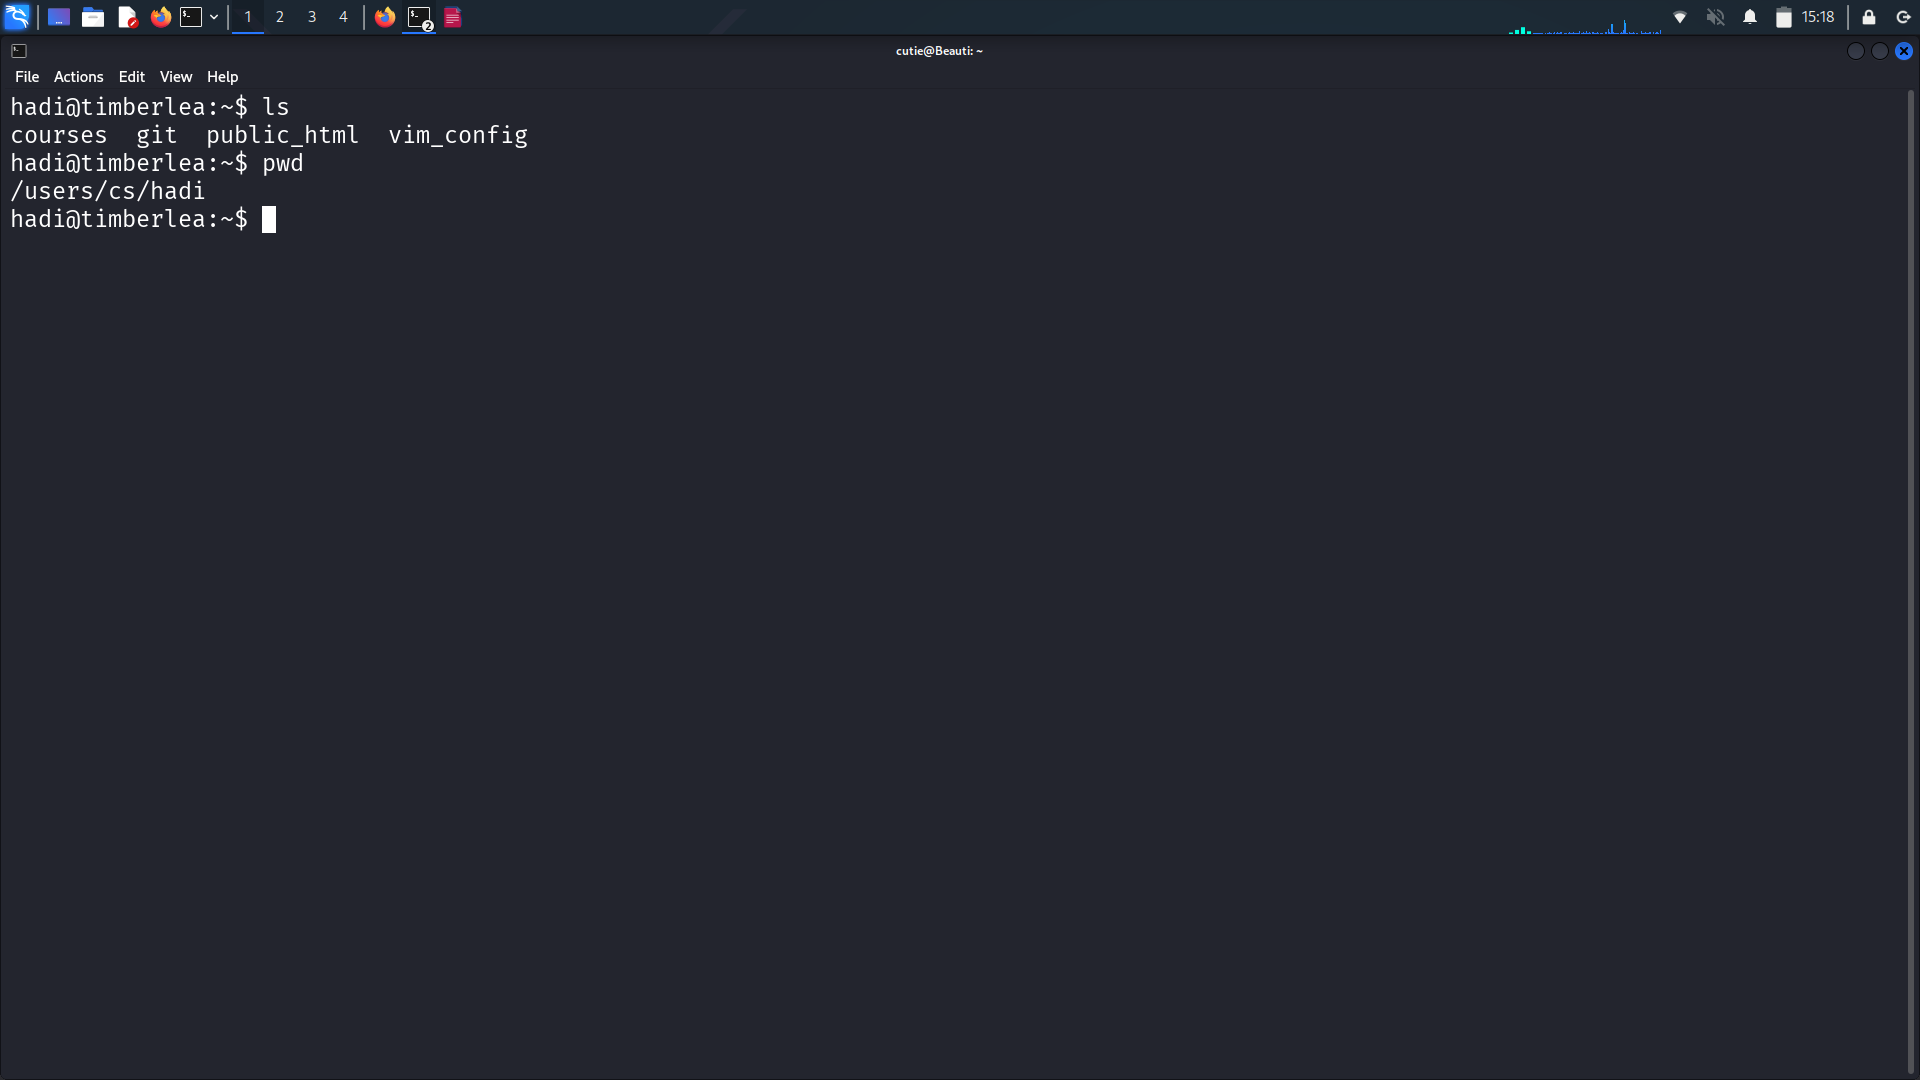
\includegraphics[width=450pt]{images/e1qA/1.png}
	\end{figure}
	
	\begin{figure}[H]
		\caption{Steps 2 and 3}
		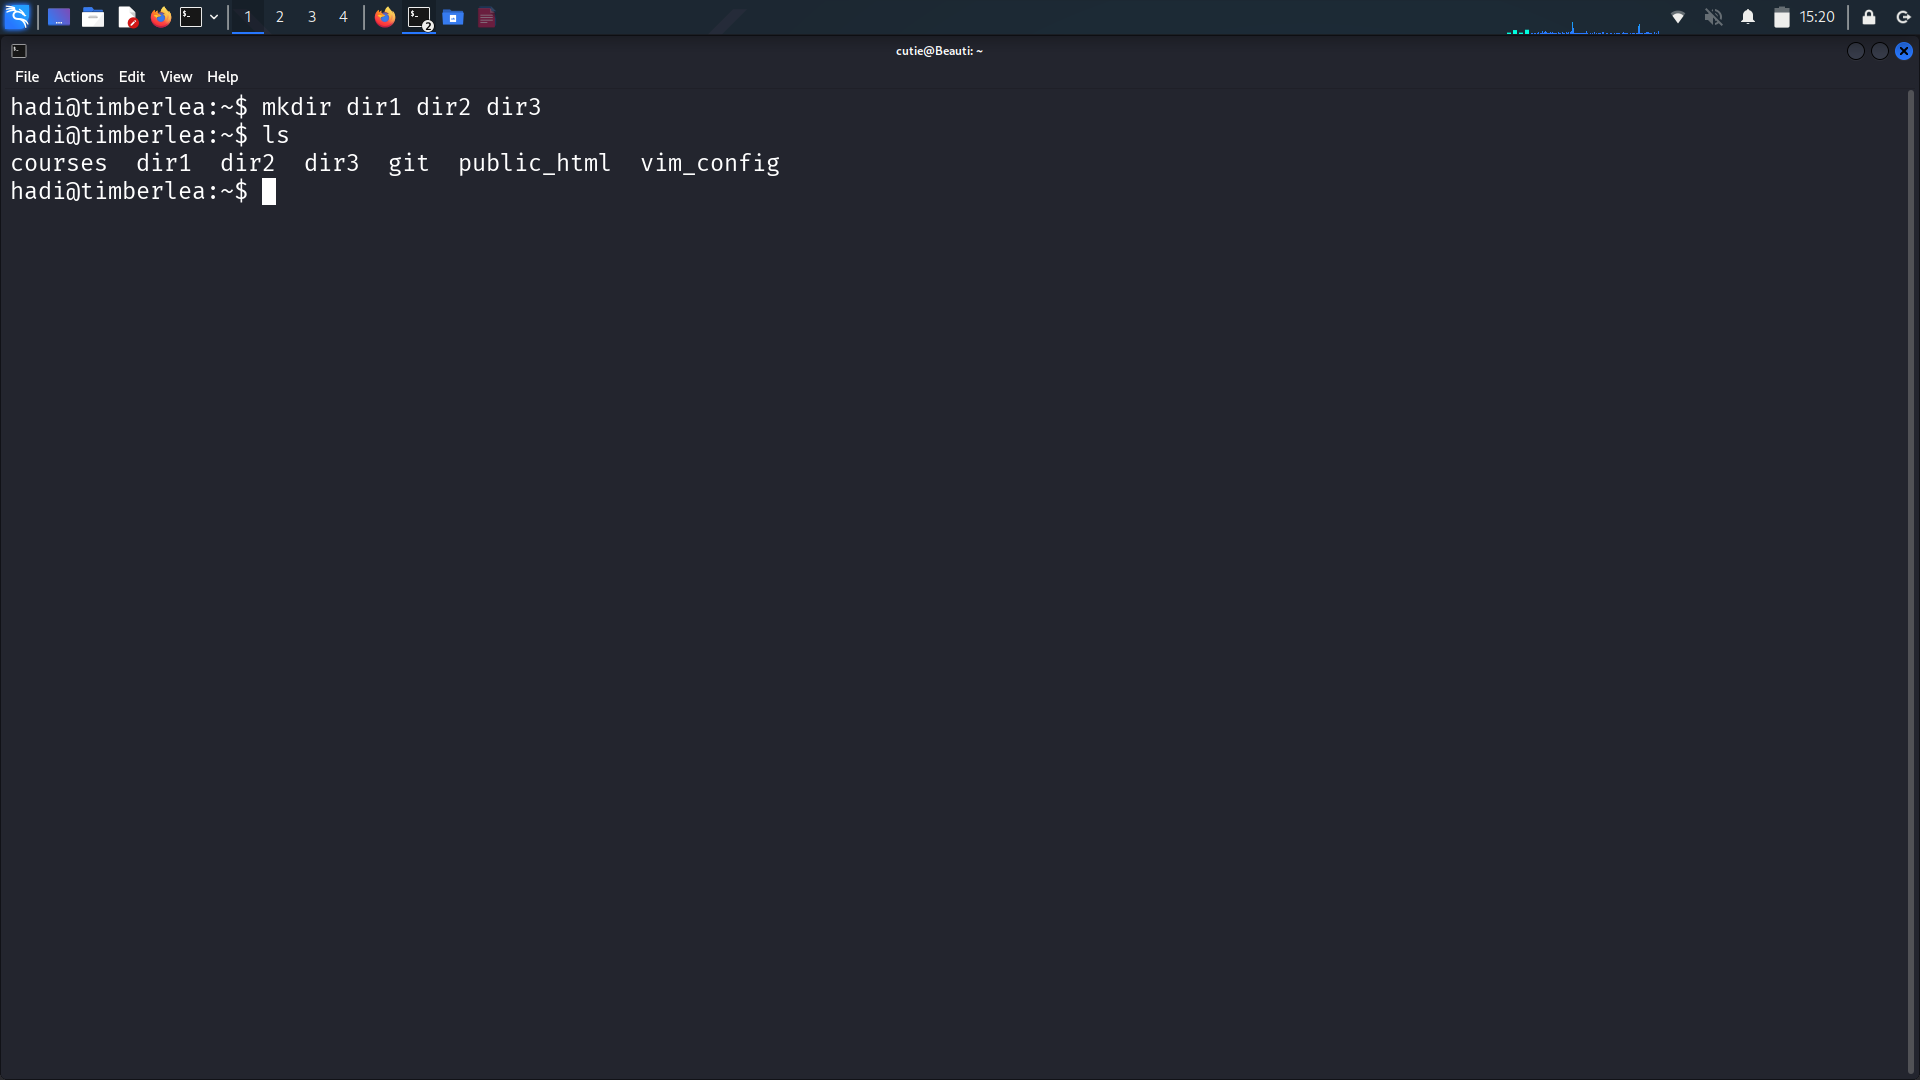
\includegraphics[width=450pt]{images/e1qA/2.png}
	\end{figure}
	\begin{figure}[H]
		\caption{Steps 4 and 5}
		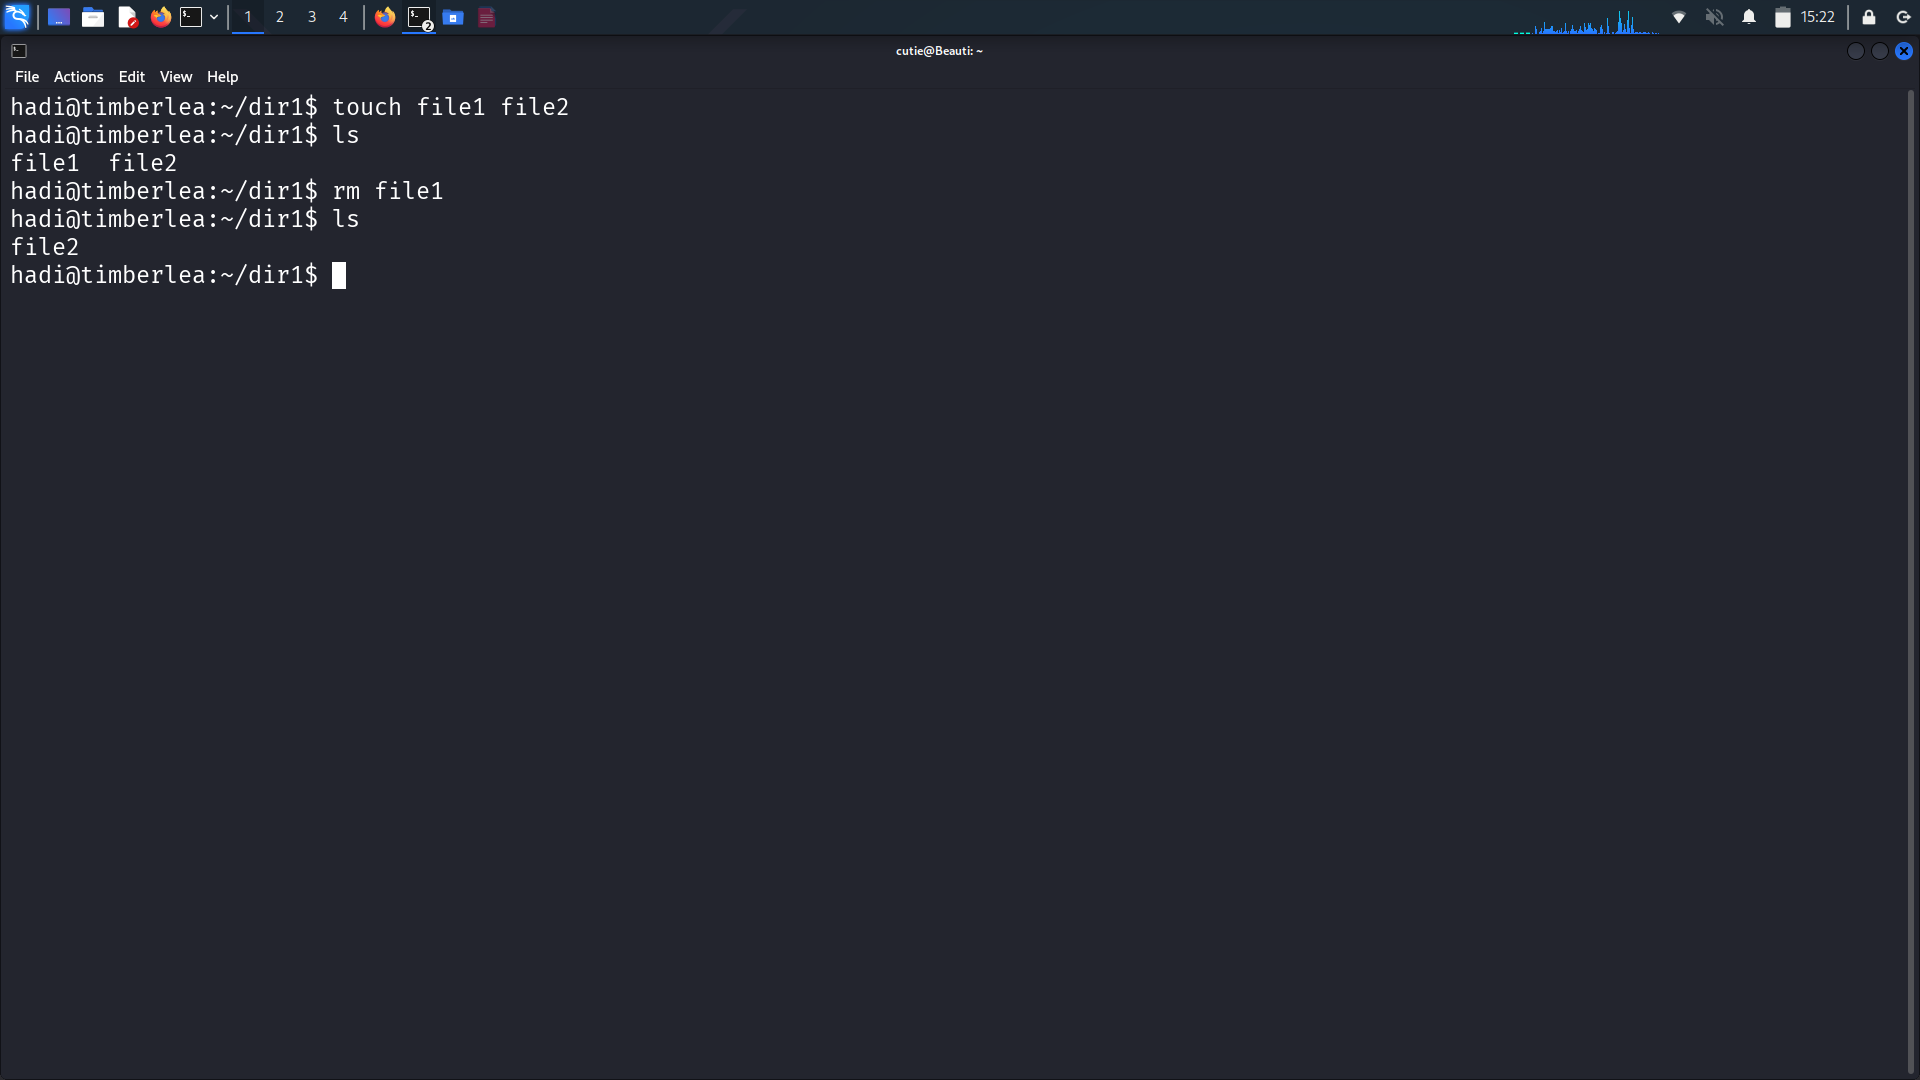
\includegraphics[width=450pt]{images/e1qA/4.png}
	\end{figure}

	\begin{figure}[H]
		\caption{Step 6}
		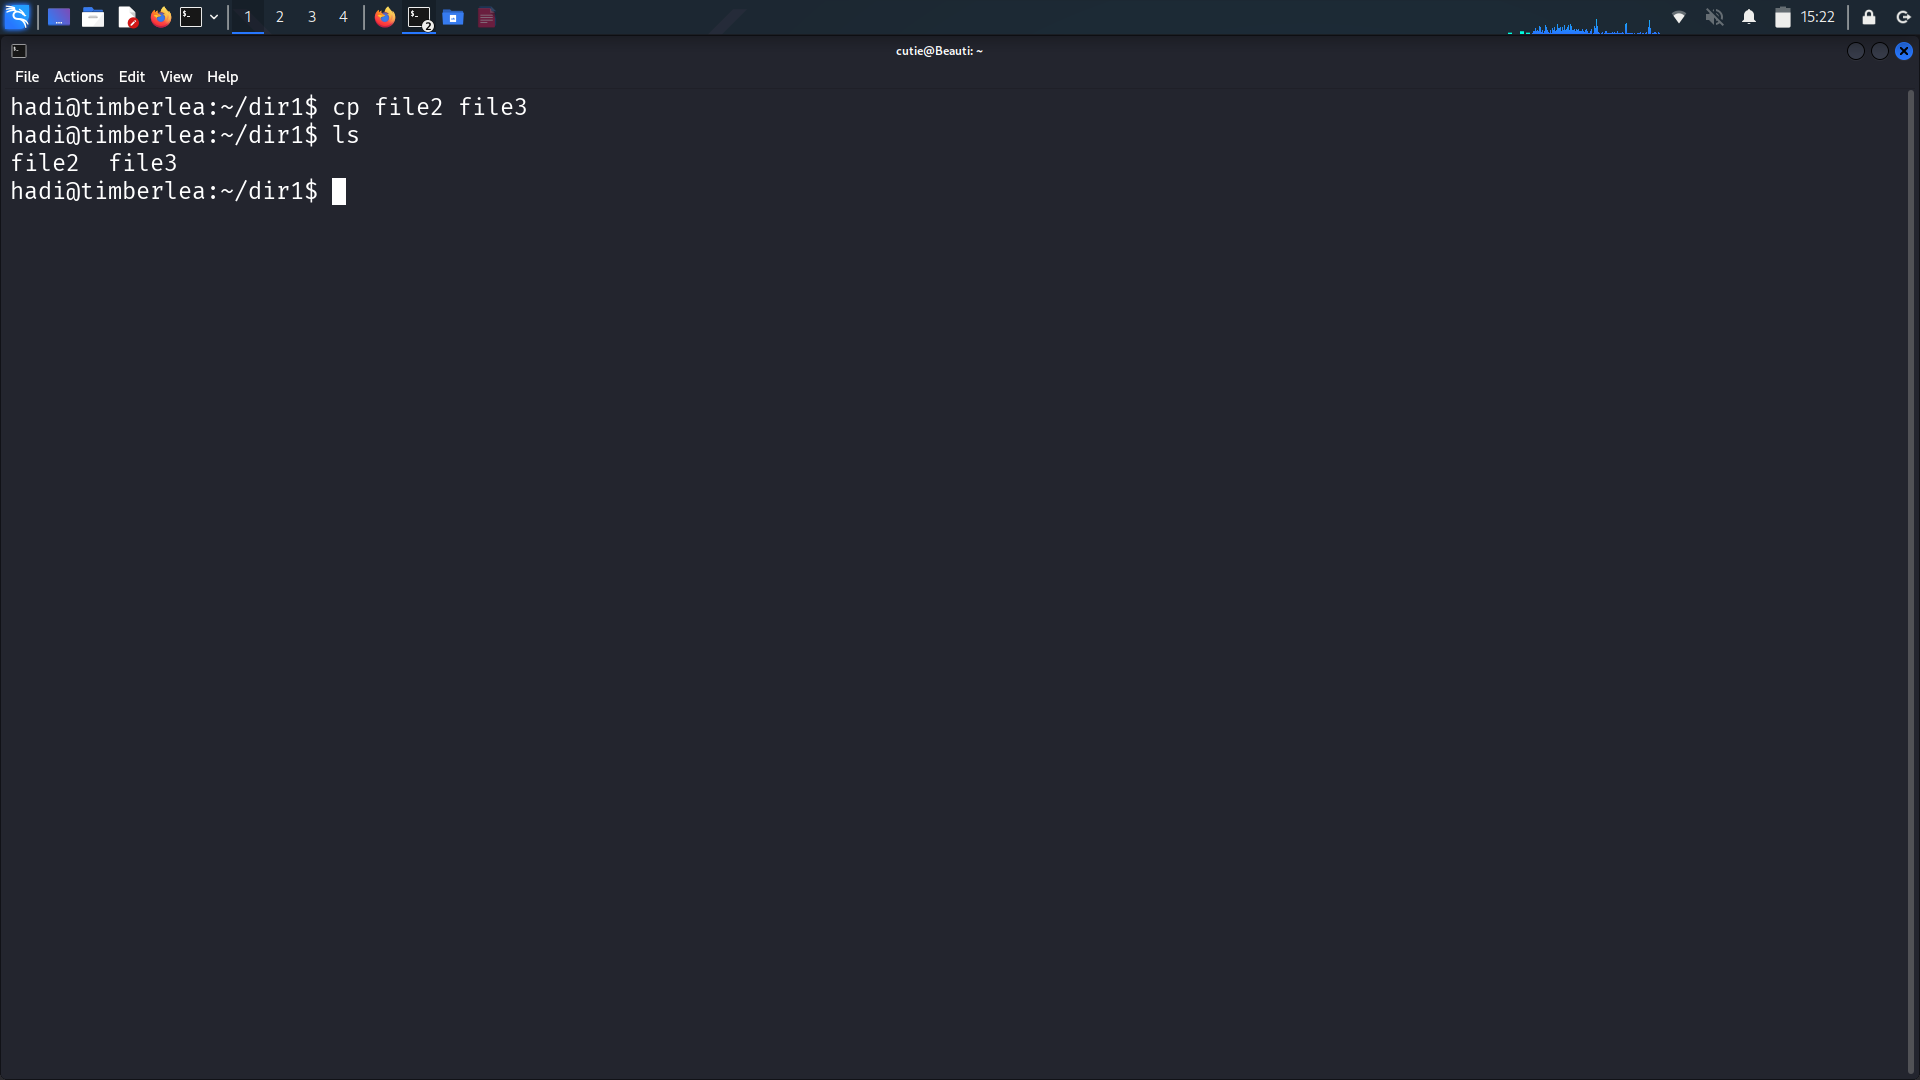
\includegraphics[width=450pt]{images/e1qA/5.png}
	\end{figure}
	\begin{figure}[H]
		\caption{Step 7}
		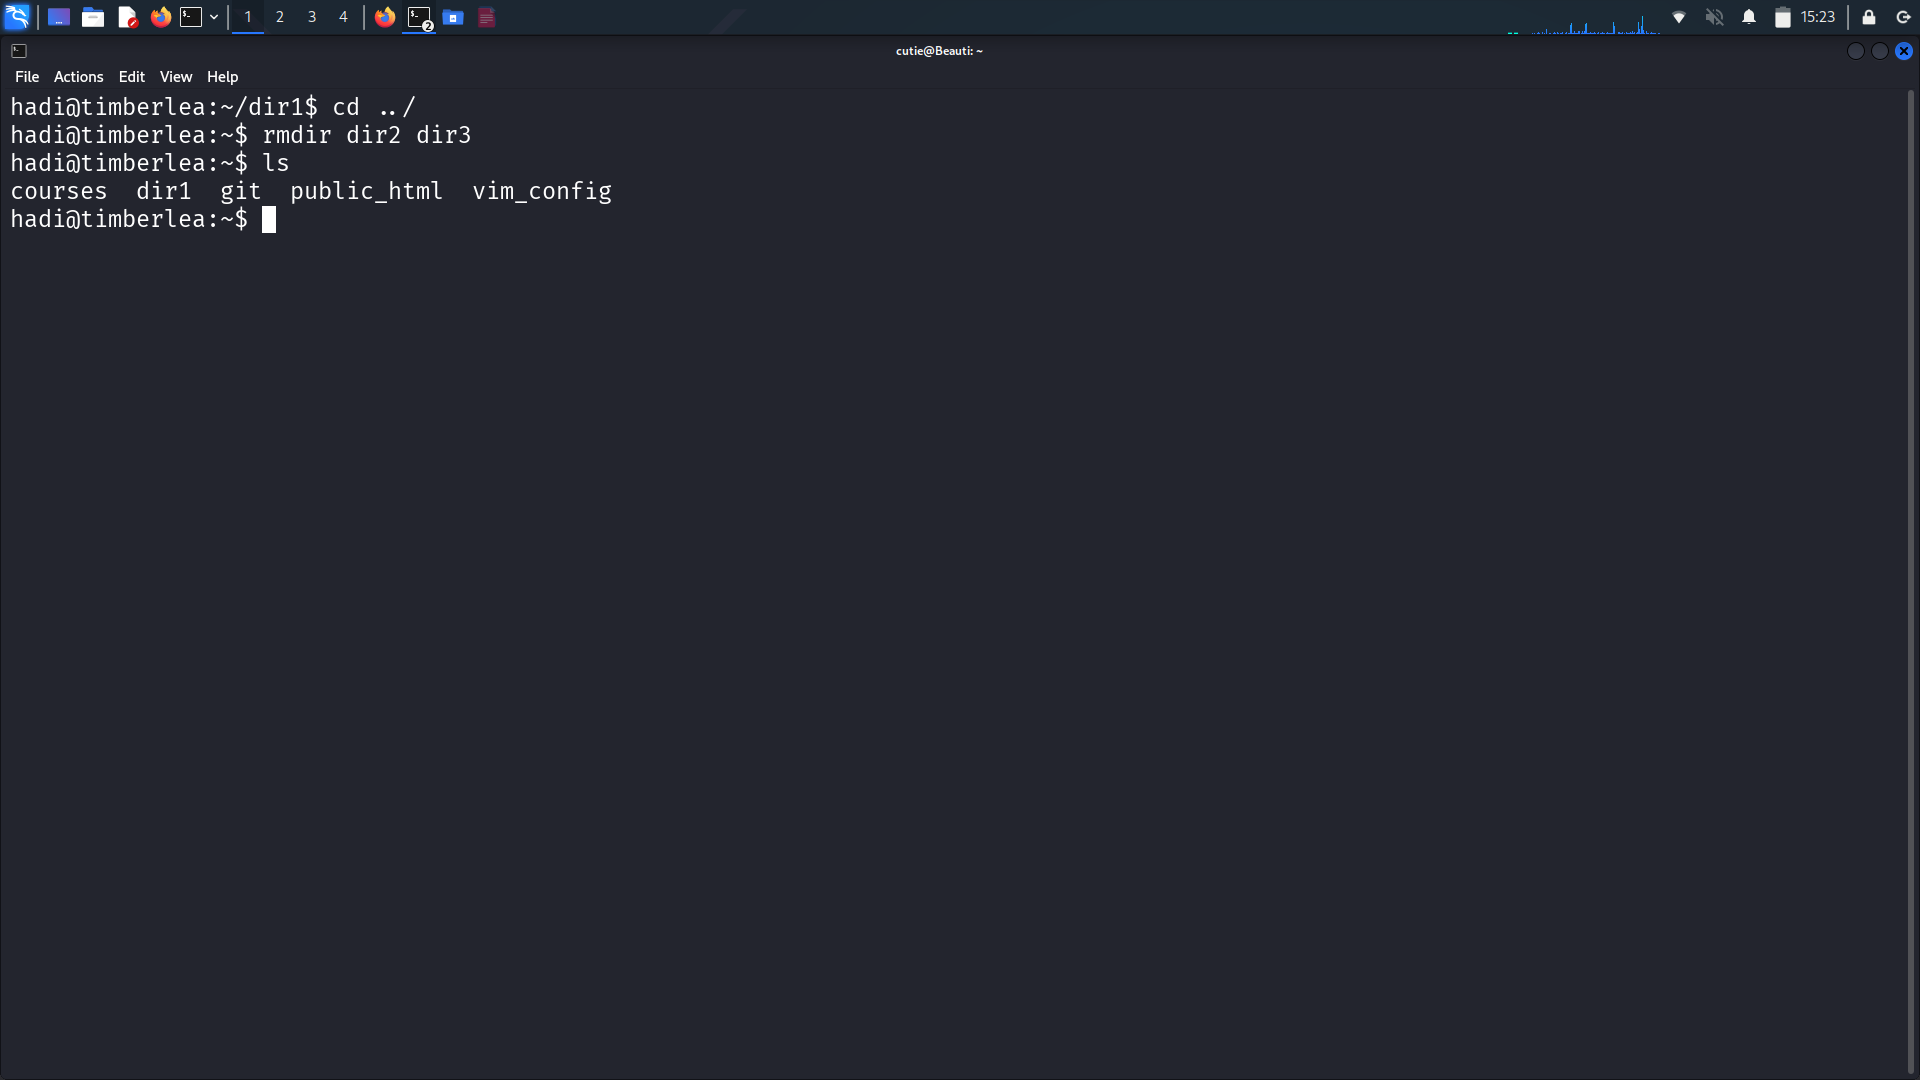
\includegraphics[width=450pt]{images/e1qA/6.png}
	\end{figure}

	\begin{figure}[H]
		\caption{Step 8}
		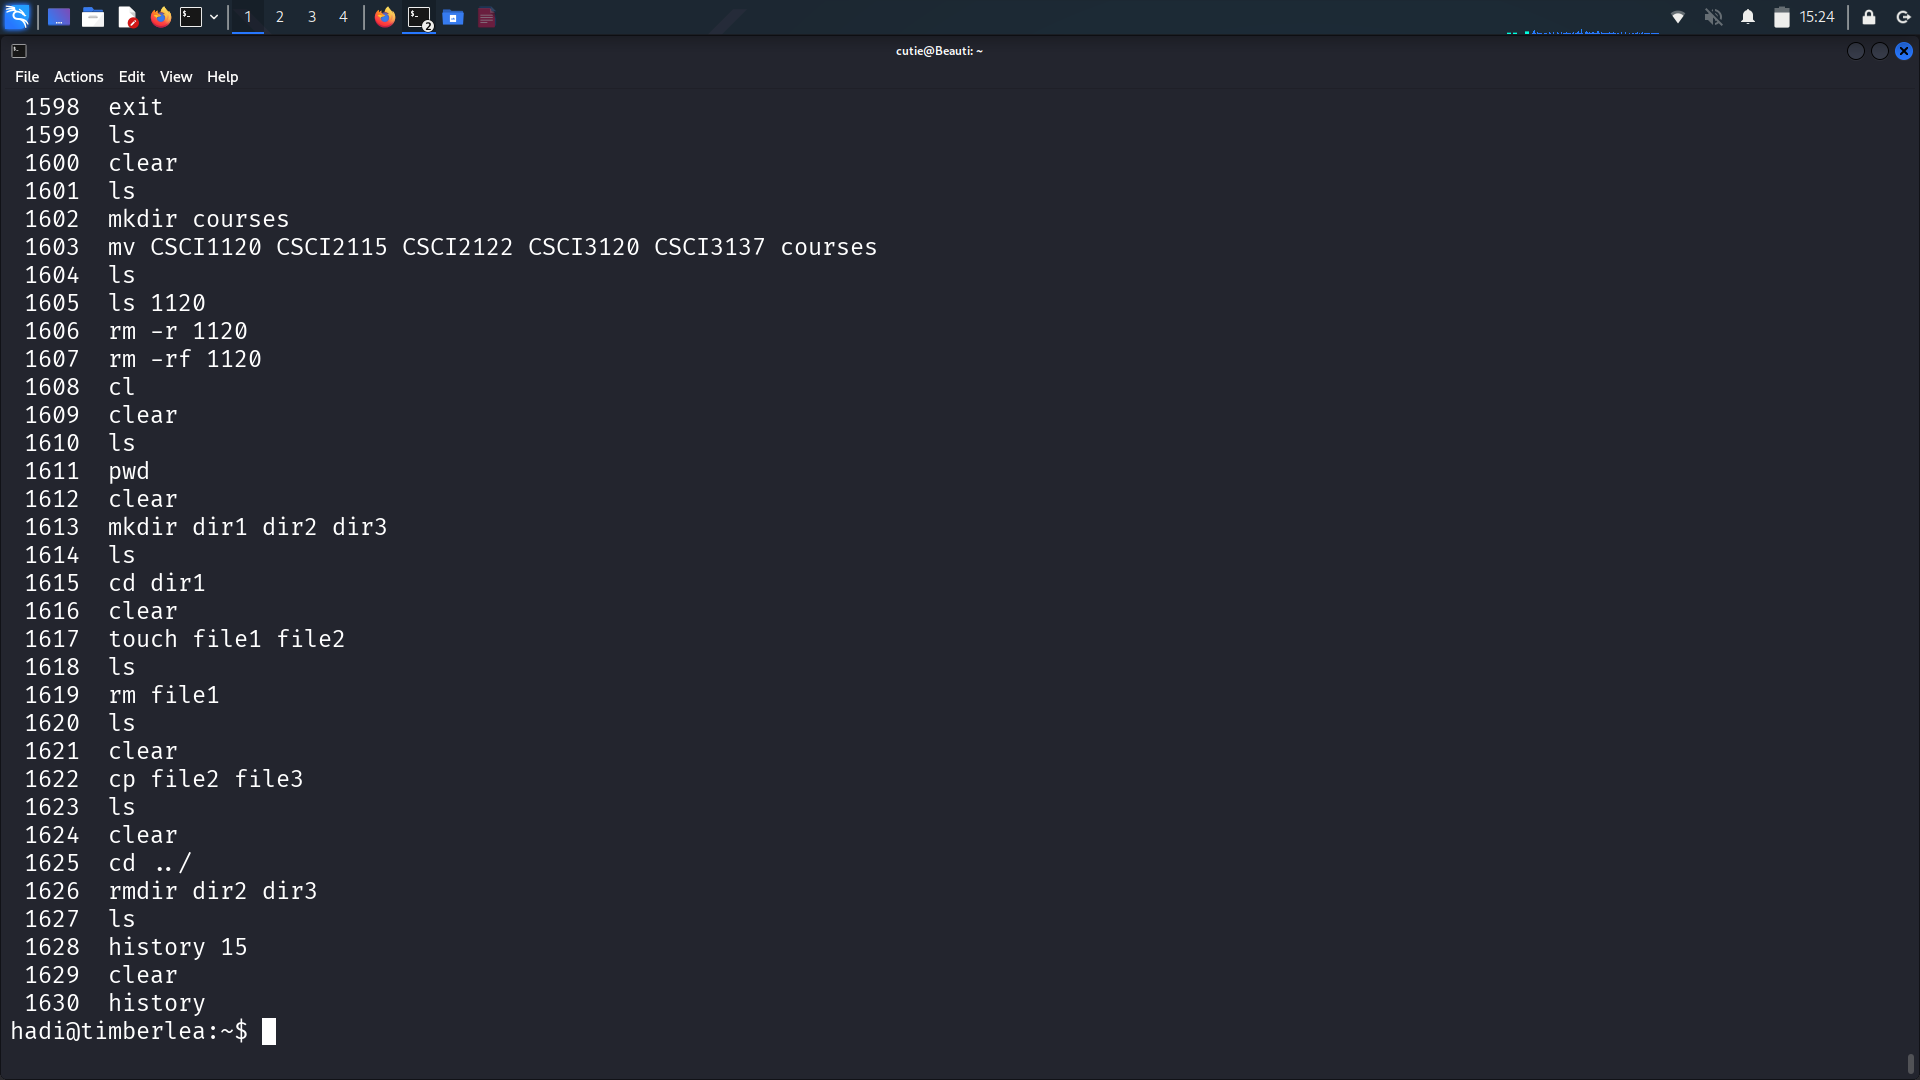
\includegraphics[width=450pt]{images/e1qA/7.png}
	\end{figure}


	\newpage
	\section{Exercise 1.B}
	\begin{figure}[H]
		\caption{Steps 1 and 2}
		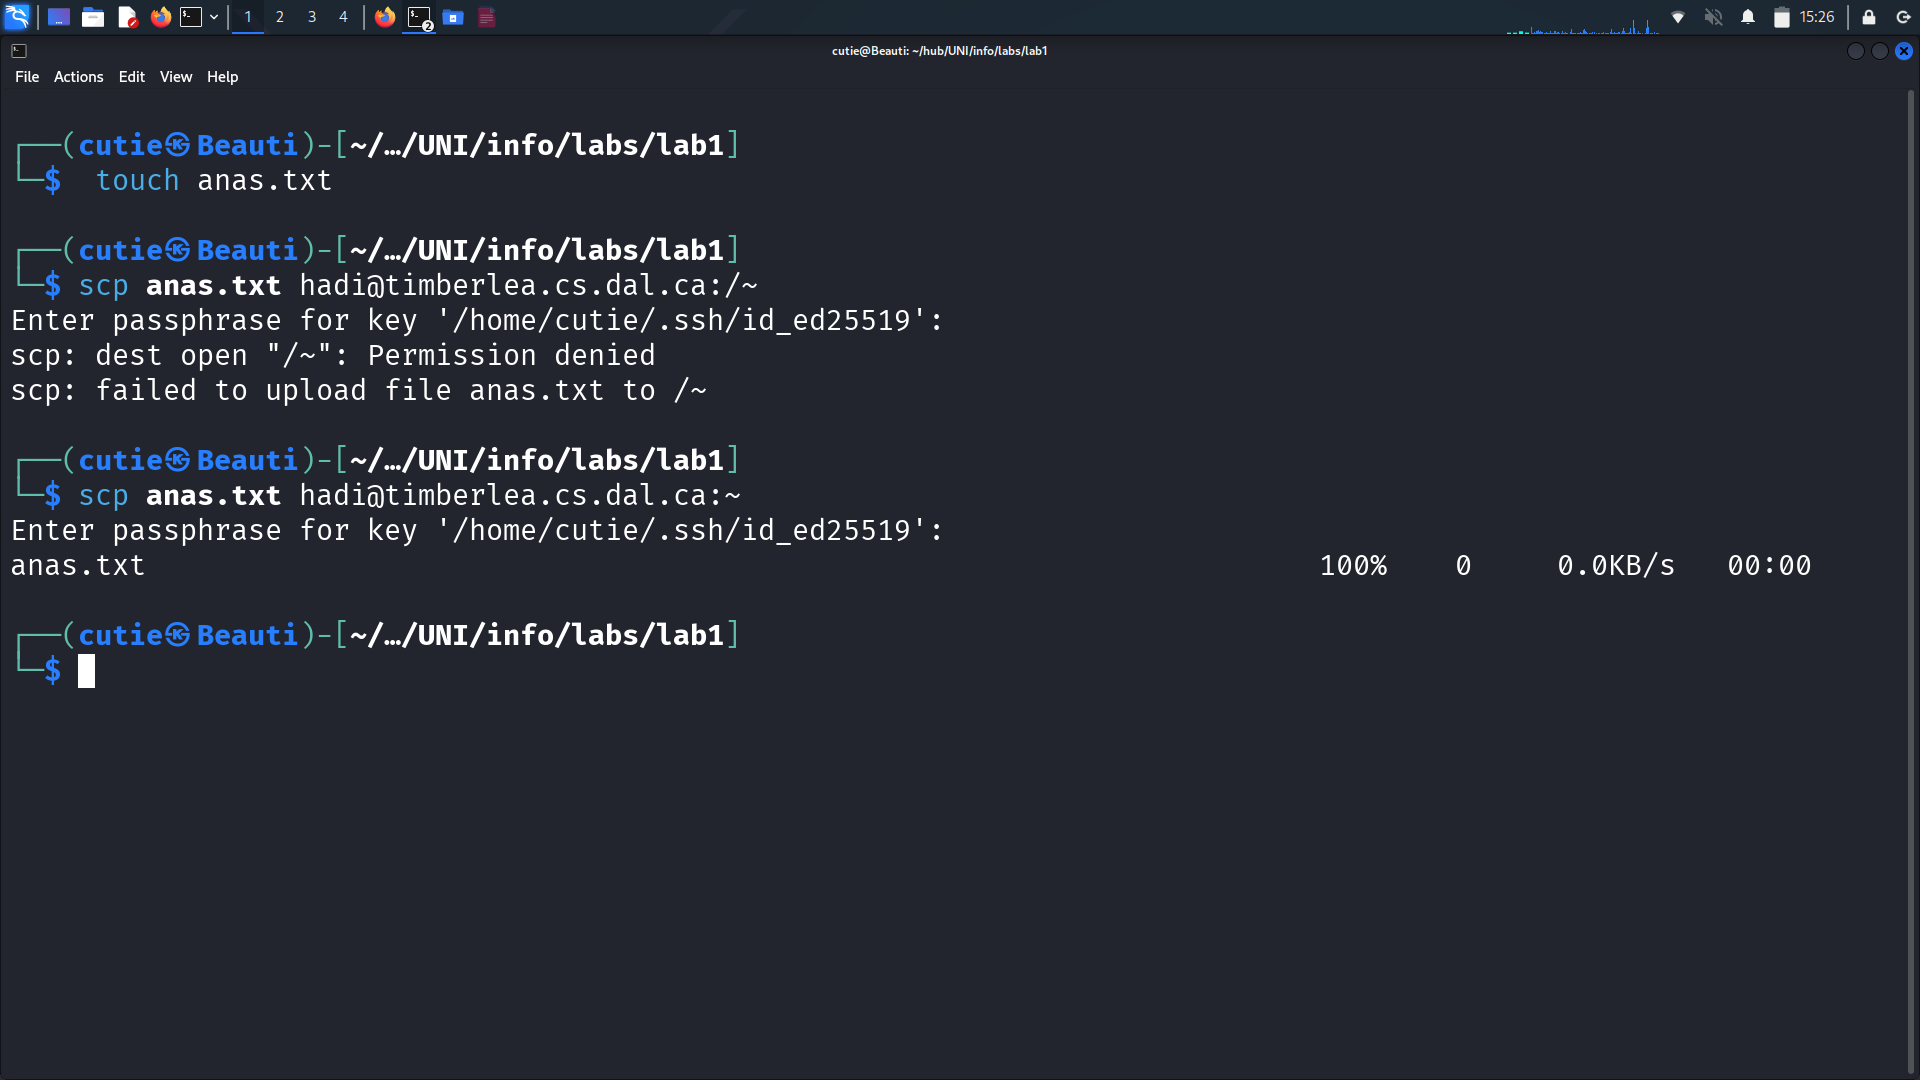
\includegraphics[width=450pt]{images/e1qB/1.png}
	\end{figure}	

	\begin{figure}[H]
		\caption{Step 3}
		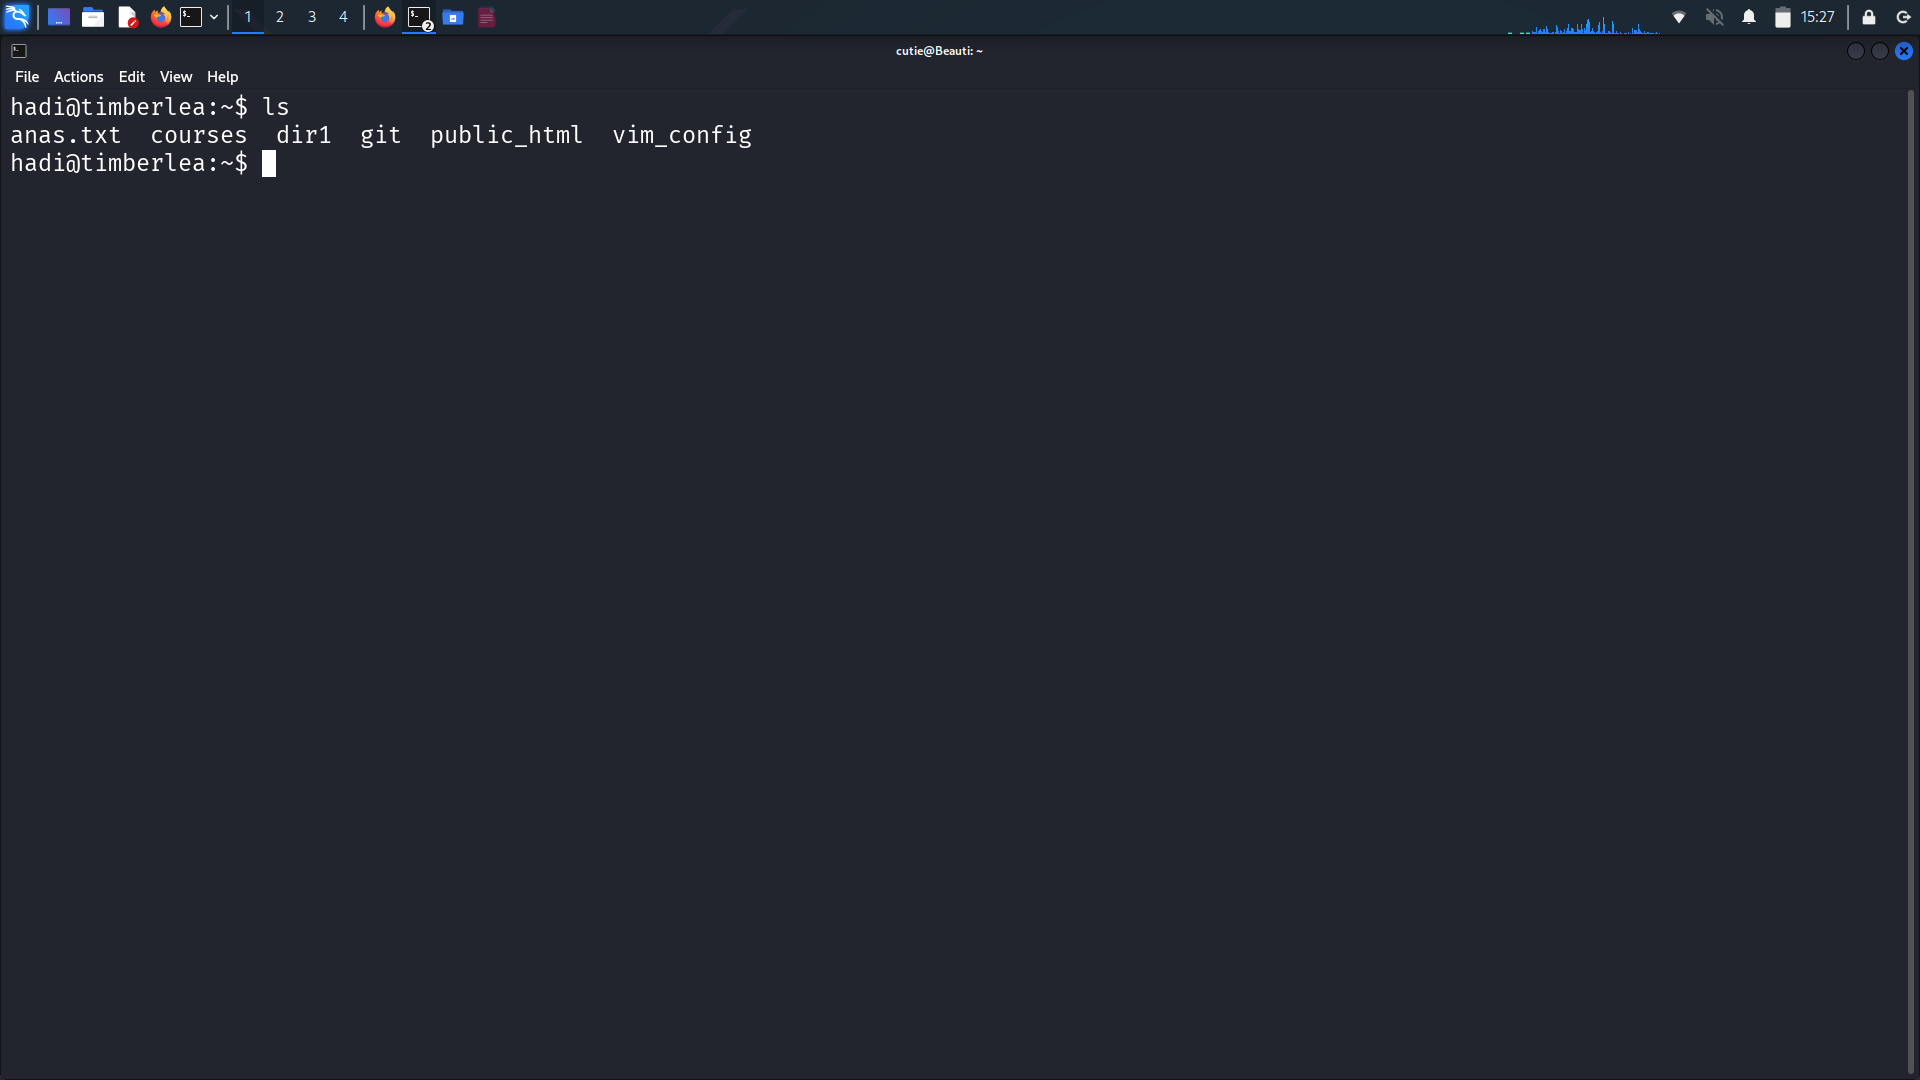
\includegraphics[width=450pt]{images/e1qB/2.png}
	\end{figure}	


	\newpage
	\section{Exercise 2.A}
	\begin{figure}[H]
		\caption{Step}
		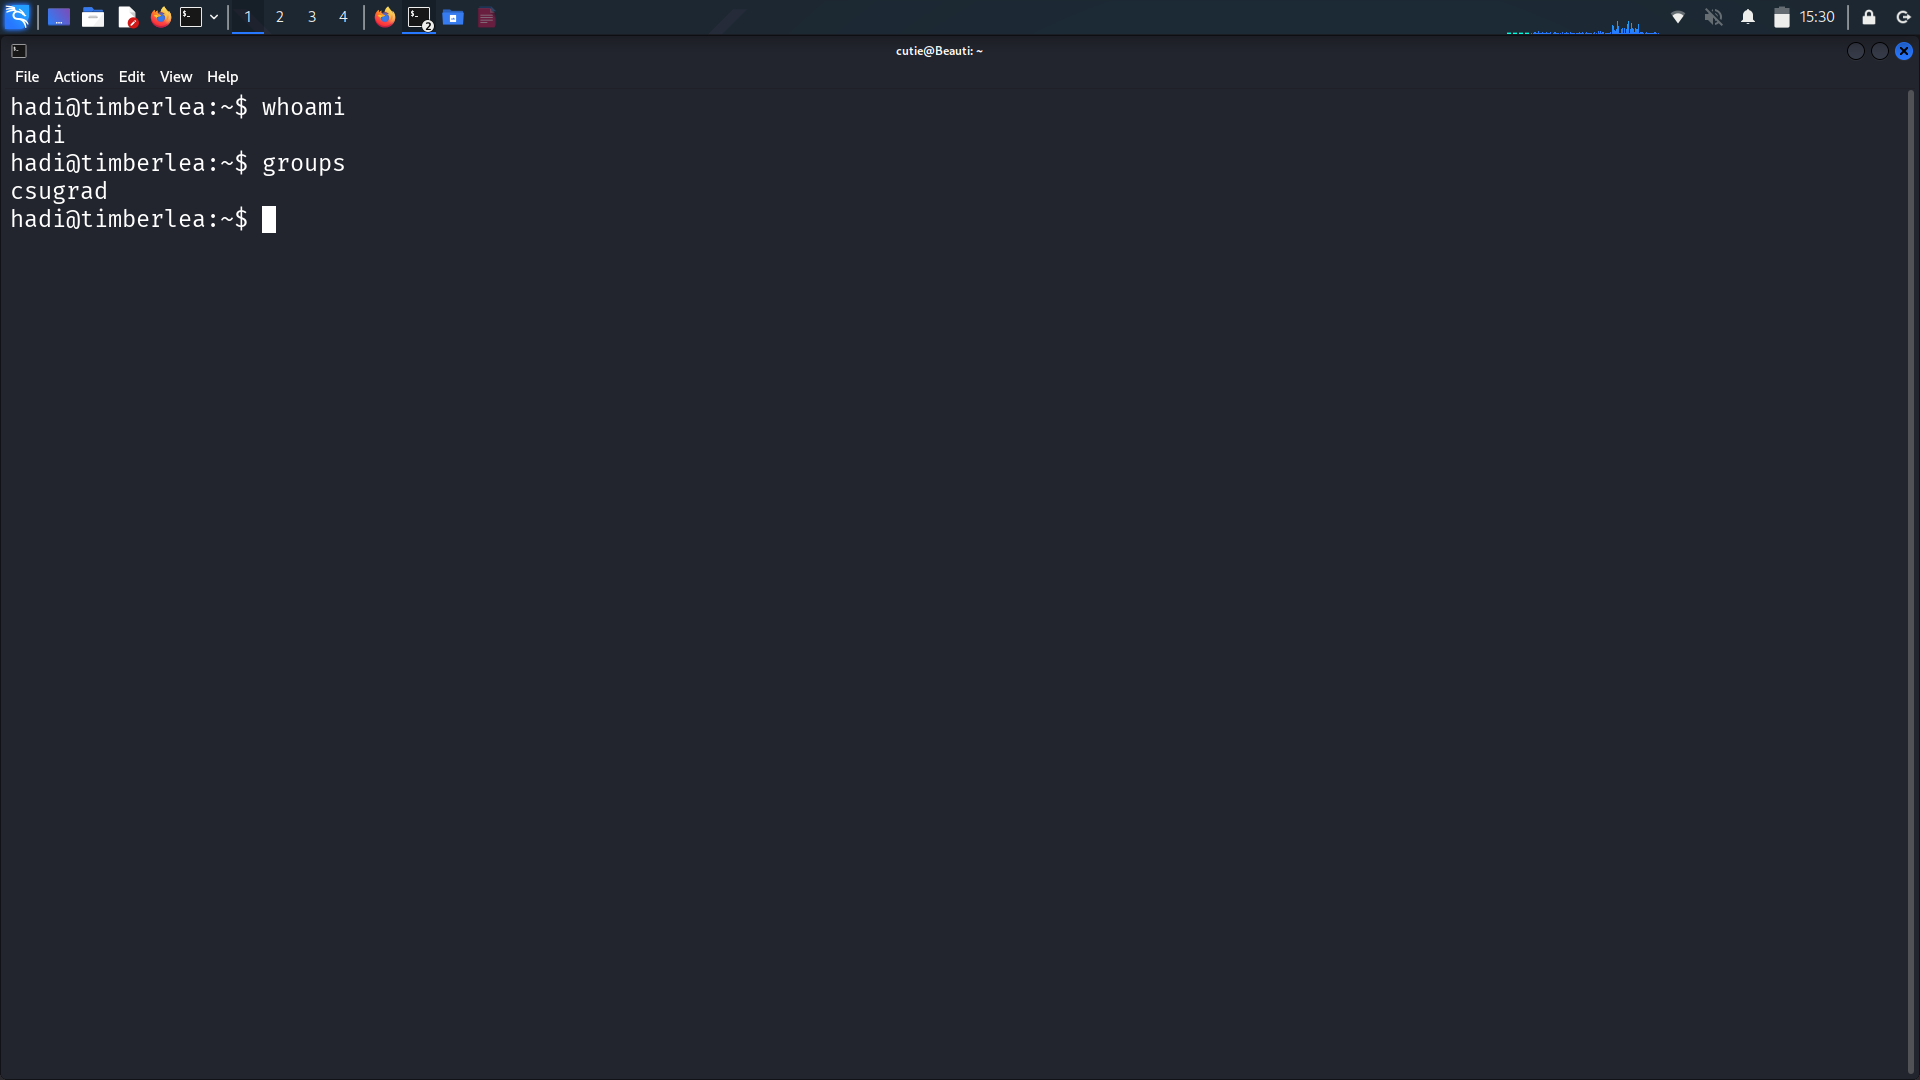
\includegraphics[width=450pt]{images/e2qA/1.png}
	\end{figure}	
	
	\begin{figure}[H]
		\caption{Step}
		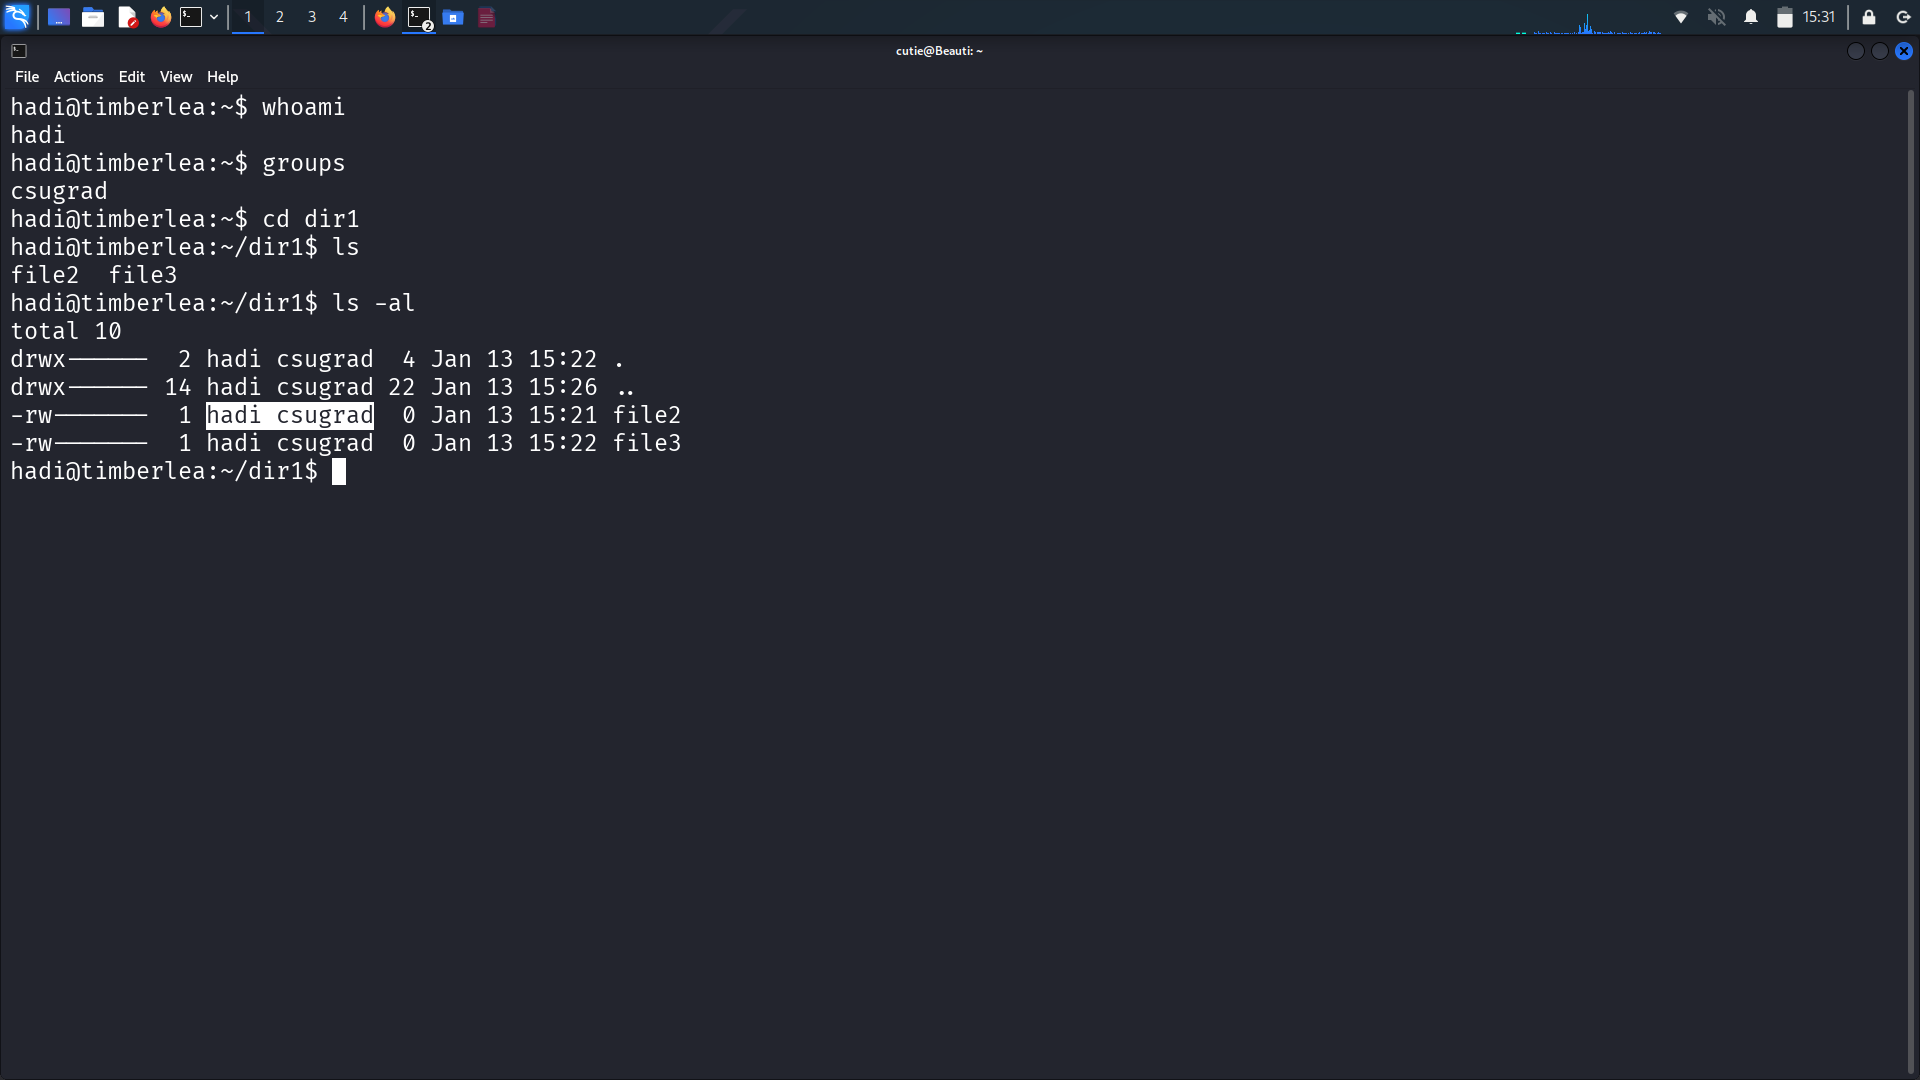
\includegraphics[width=450pt]{images/e2qA/2.png}
	\end{figure}

	\par{
		the \textbf{whoami} and \textbf{groups} commands do not take file names as
		arguments and return an error. whoami does not expect any user argument and
		only returns the name of the effective userID. groups can take a username
		as an argument and return the groups that they are a part of.
	
	To check for the group and owner of a file we can run ls -al $<$file\_name$>$
	}

	\newpage
	\section{Exercise 2.B}
	
	\begin{figure}[H]
		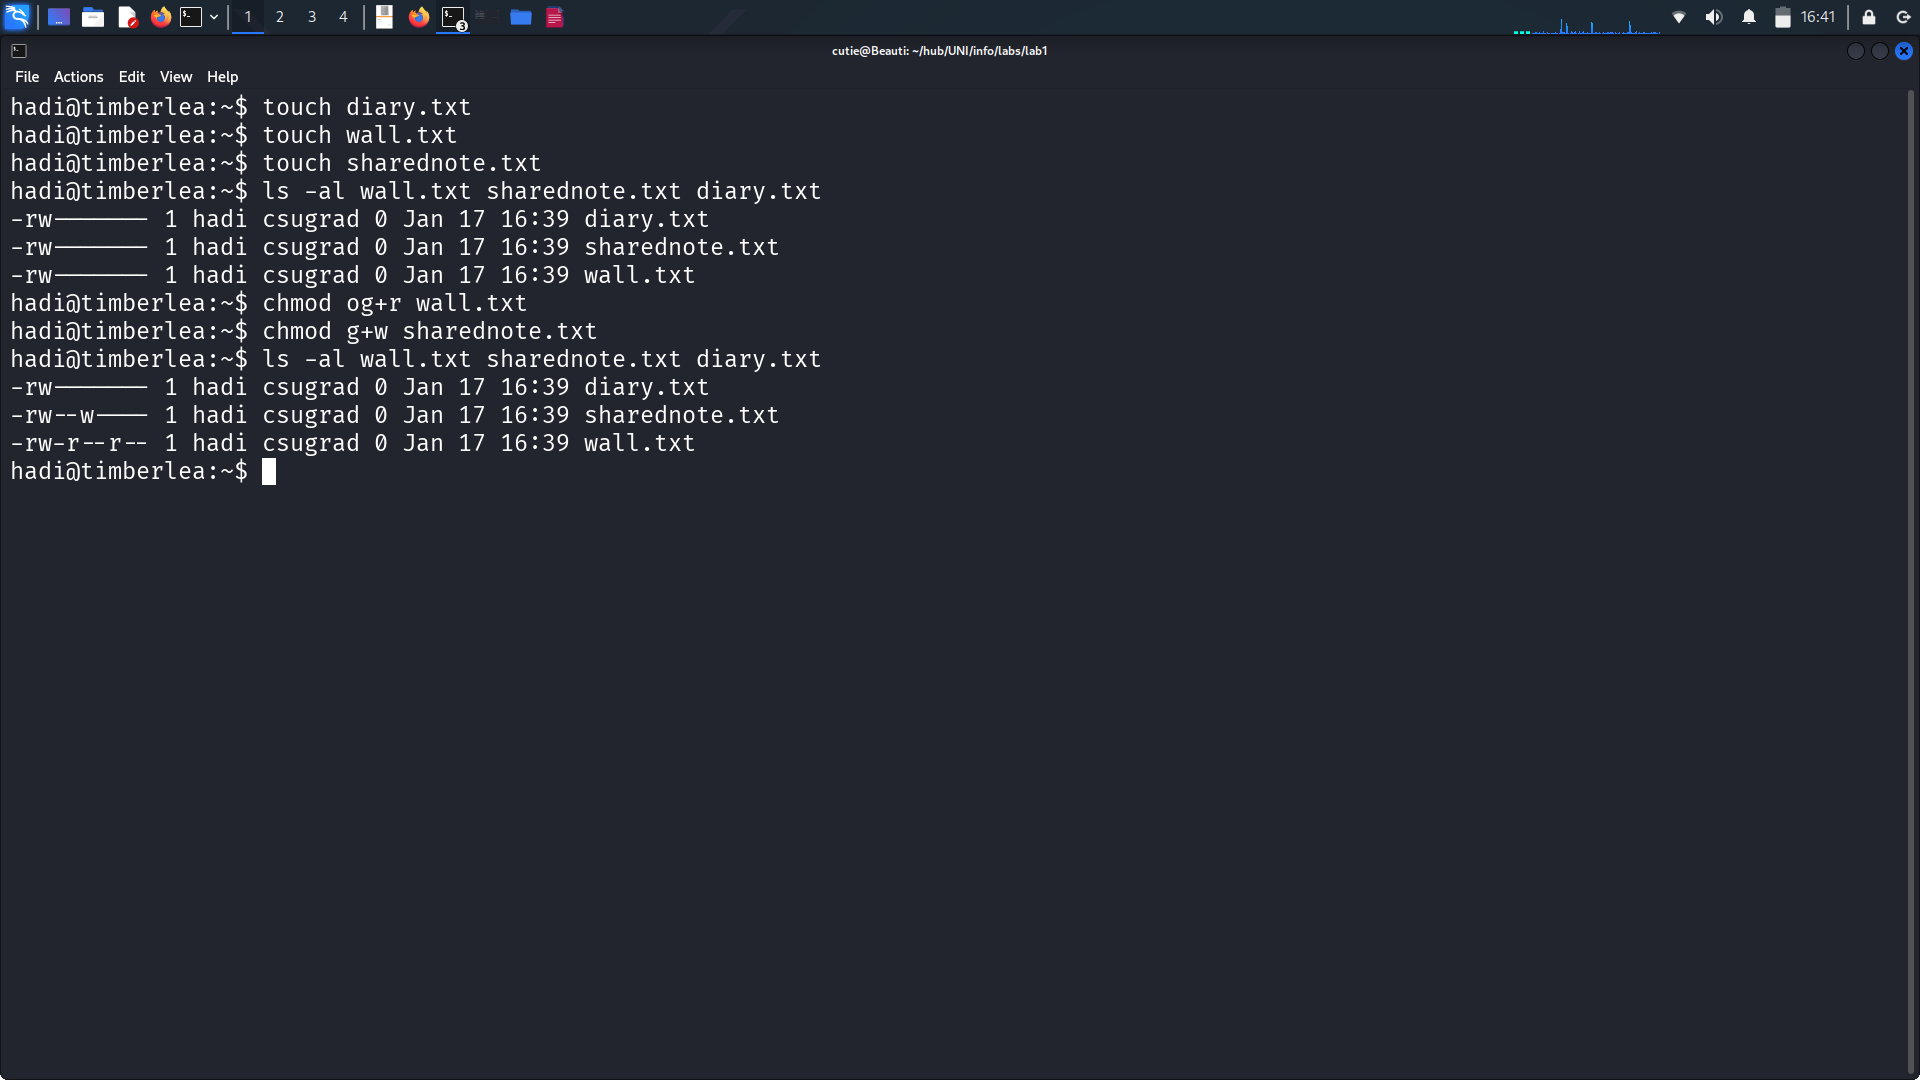
\includegraphics[width=400pt]{images/e2qB/e2.png}
	\end{figure}

	\textbf{Explaination:}
	\begin{enumerate}
		\item diary.txt: No changes to the permissions were required since only the
			user "hadi" (me) can read and write to the file

		\item wall.txt: The command i used can be reduced to only \textbf{o+r} as 
			that includes everyone but still, giving every user in the csugrad group
			and everyone else the permission to read.
		
		\item sharednote.txt: The command \textbf{g+w} assigns writing permission 
			to everyone in the group that the file is assigned to. 
	\end{enumerate}



	\newpage
	\section{Exercise 3.A}
	
	\textbf{Welcome:}

	\begin{figure}[H]
		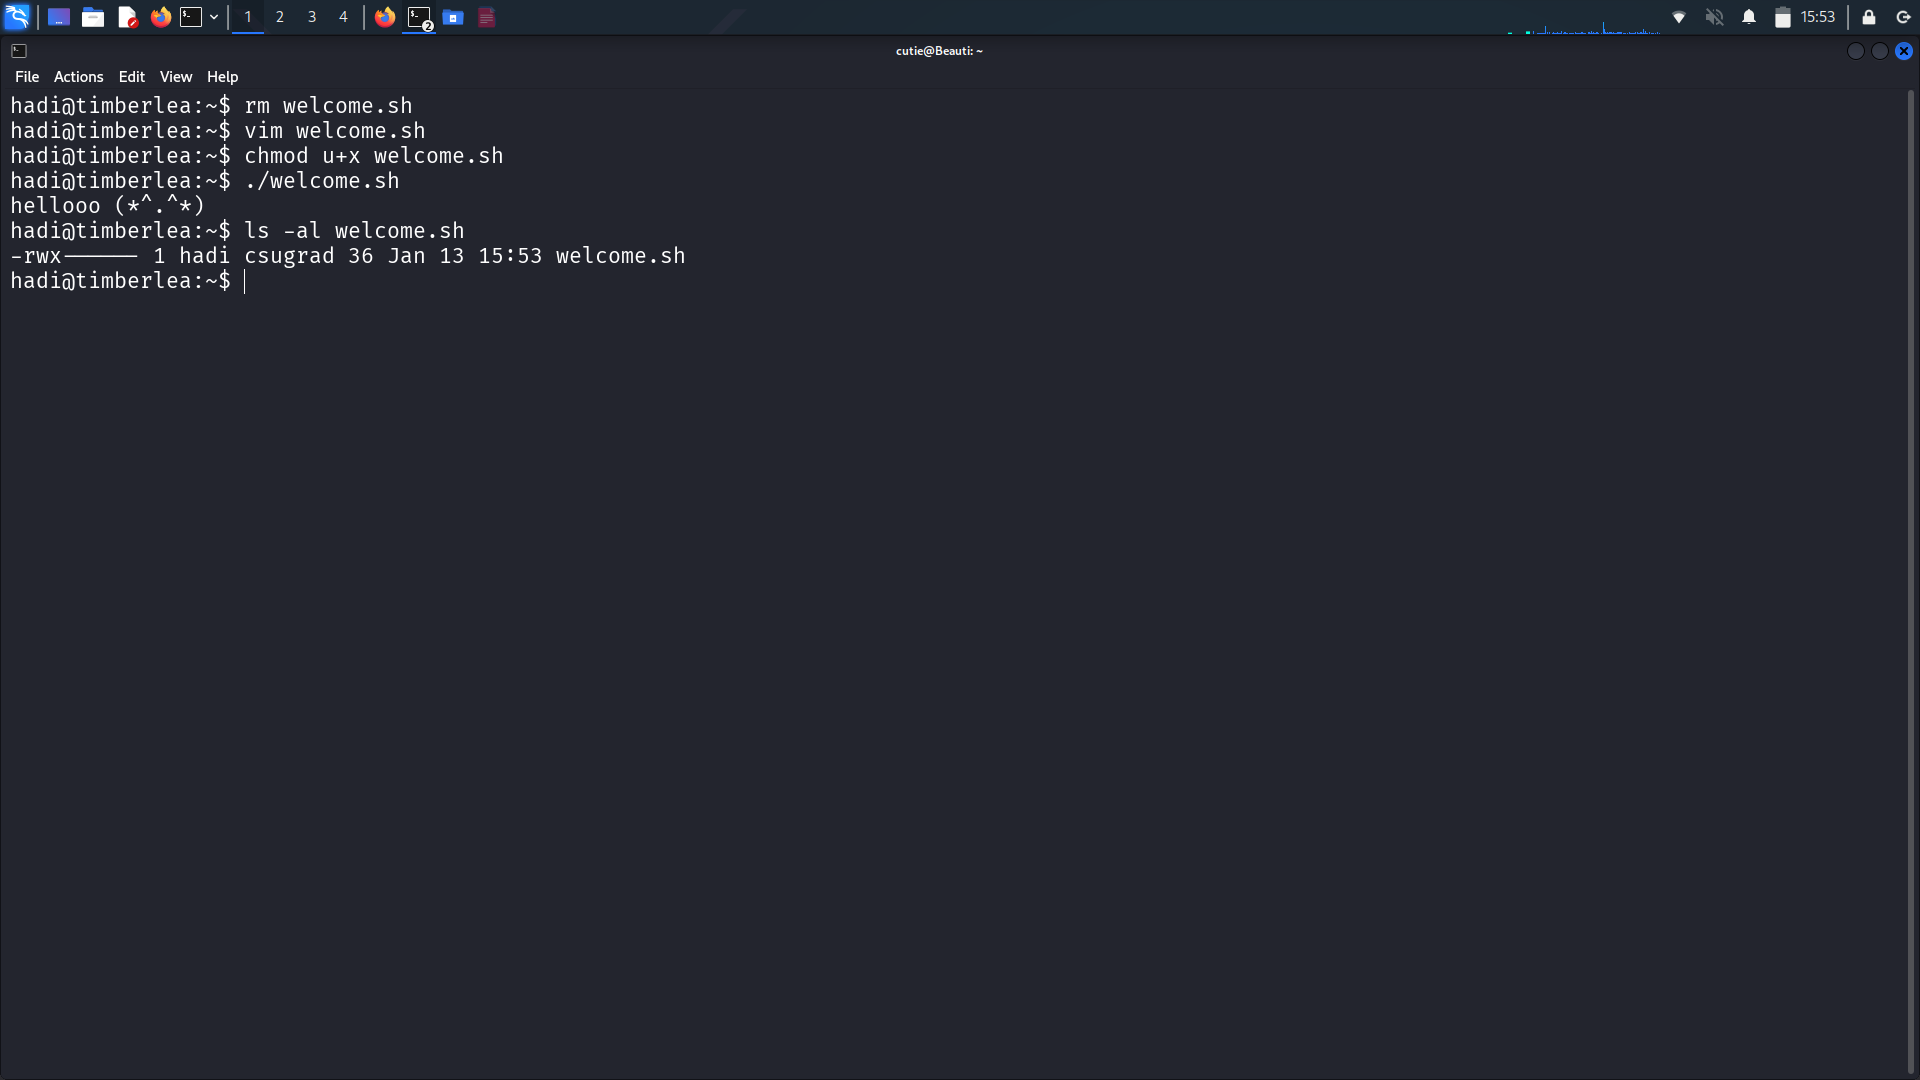
\includegraphics[width=400pt]{images/e3qA/1.png}
	\end{figure}
	\begin{figure}[H]
		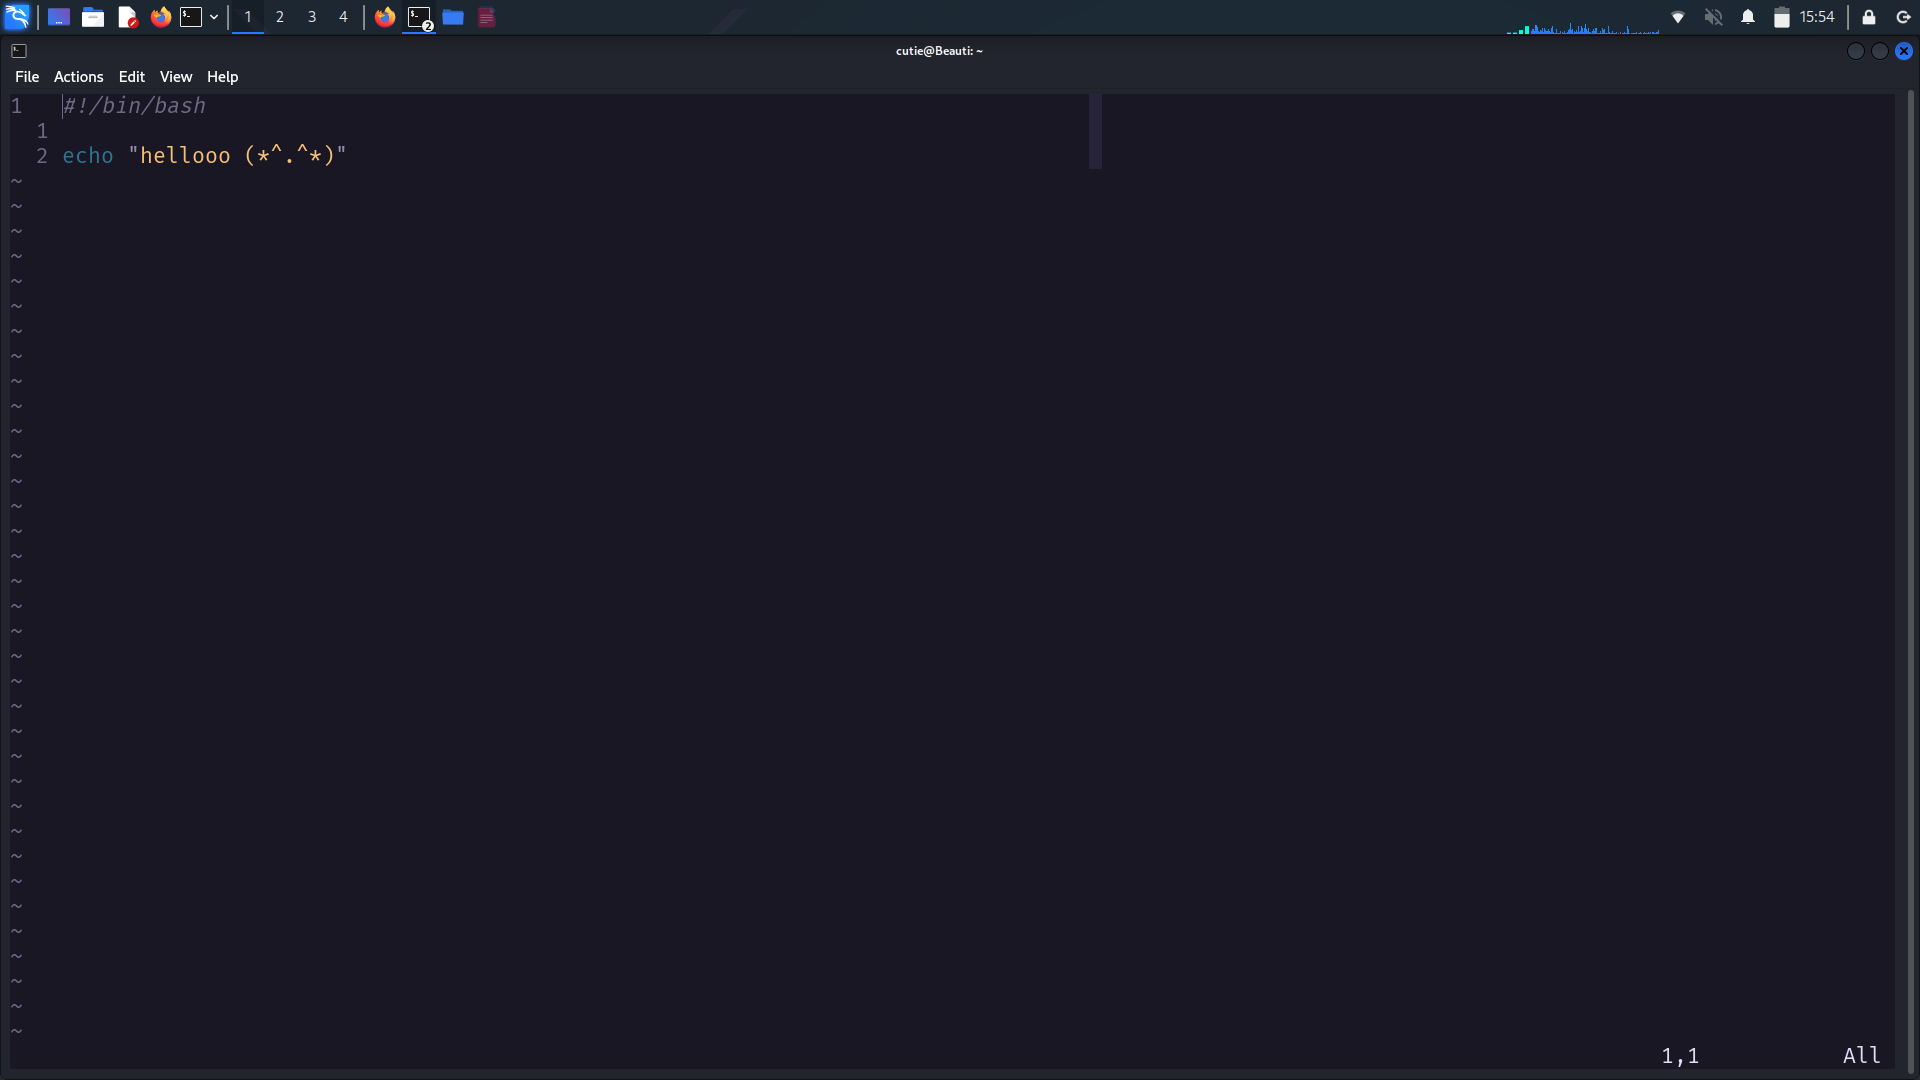
\includegraphics[width=400pt]{images/e3qA/2.png}
	\end{figure}

	\newpage
	\textbf{Warning:}
	\begin{figure}[H]
		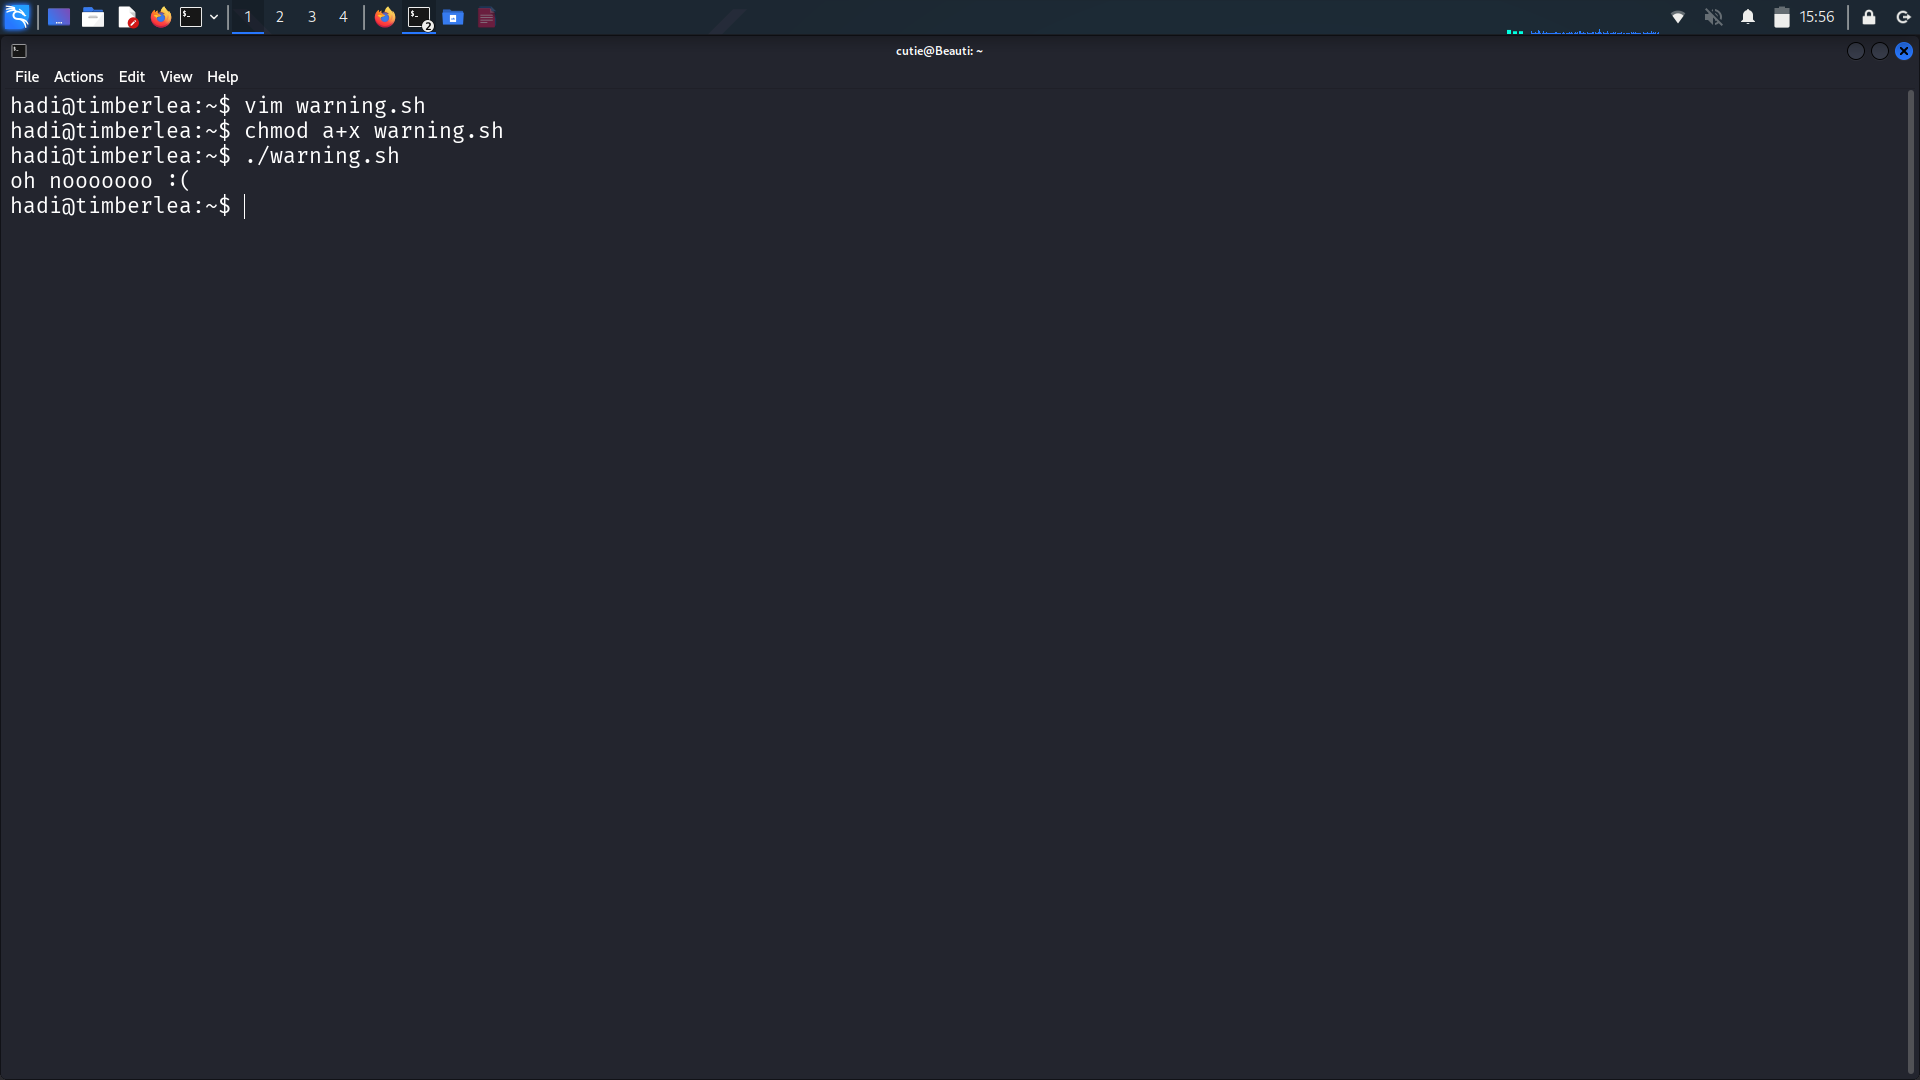
\includegraphics[width=400pt]{images/e3qA/3.png}
	\end{figure}
	\begin{figure}[H]
		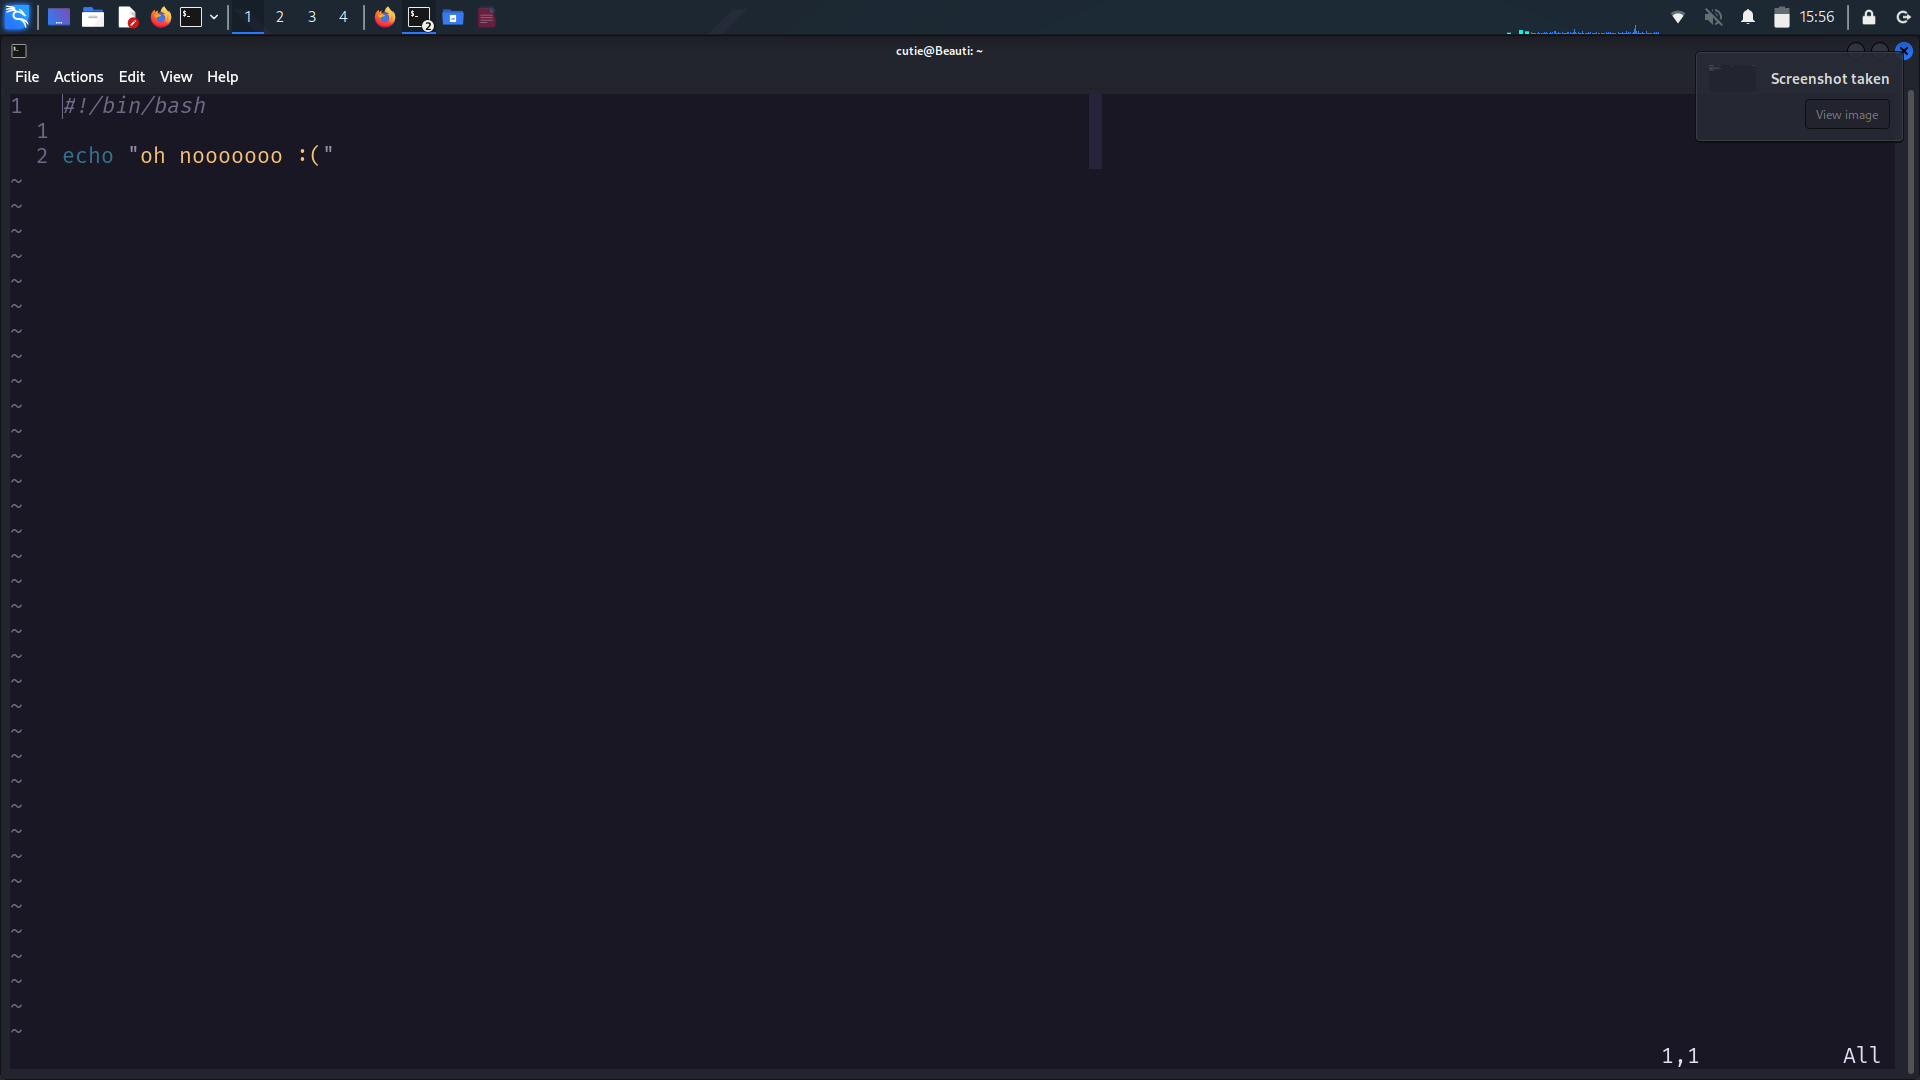
\includegraphics[width=400pt]{images/e3qA/4.png}
	\end{figure}

	\section{Exercise 3.B}
	\begin{figure}[H]
			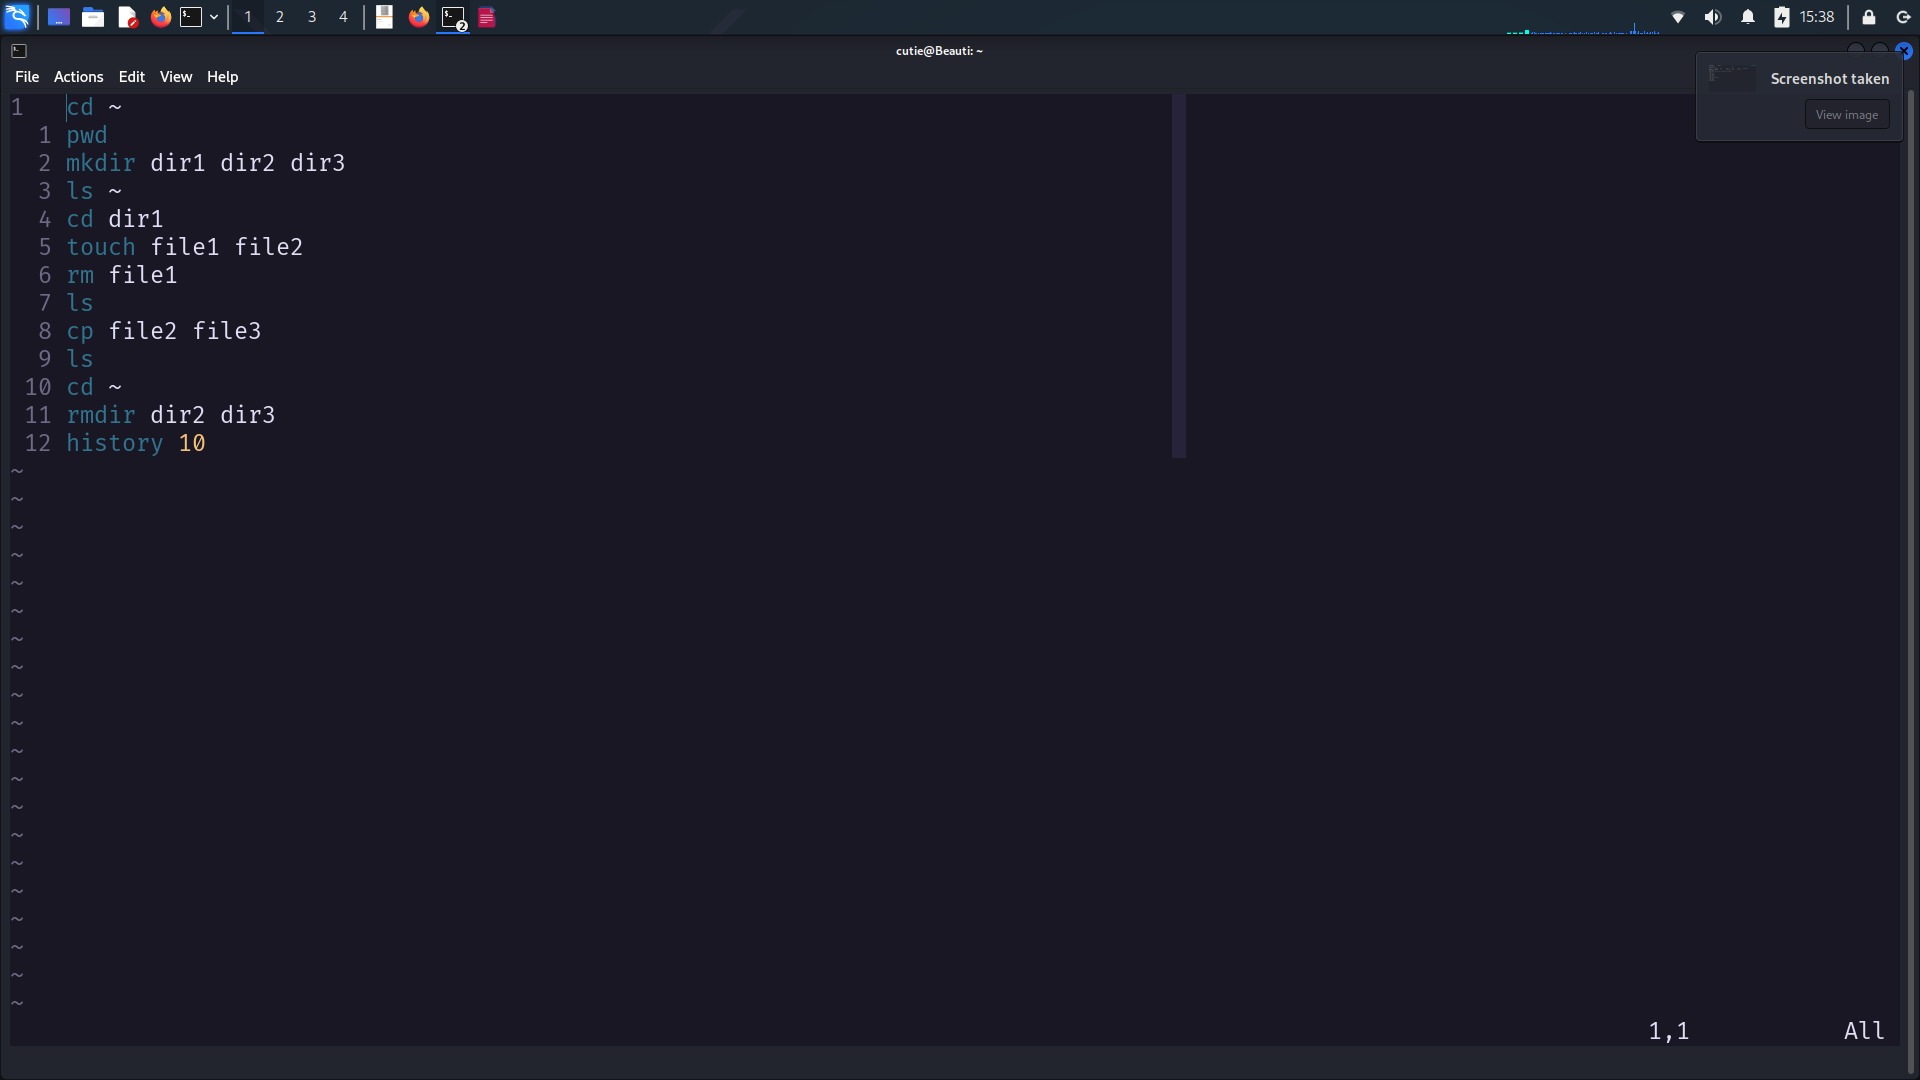
\includegraphics[width=400pt]{images/3b1.png}
	\end{figure}


	\begin{figure}[H]
			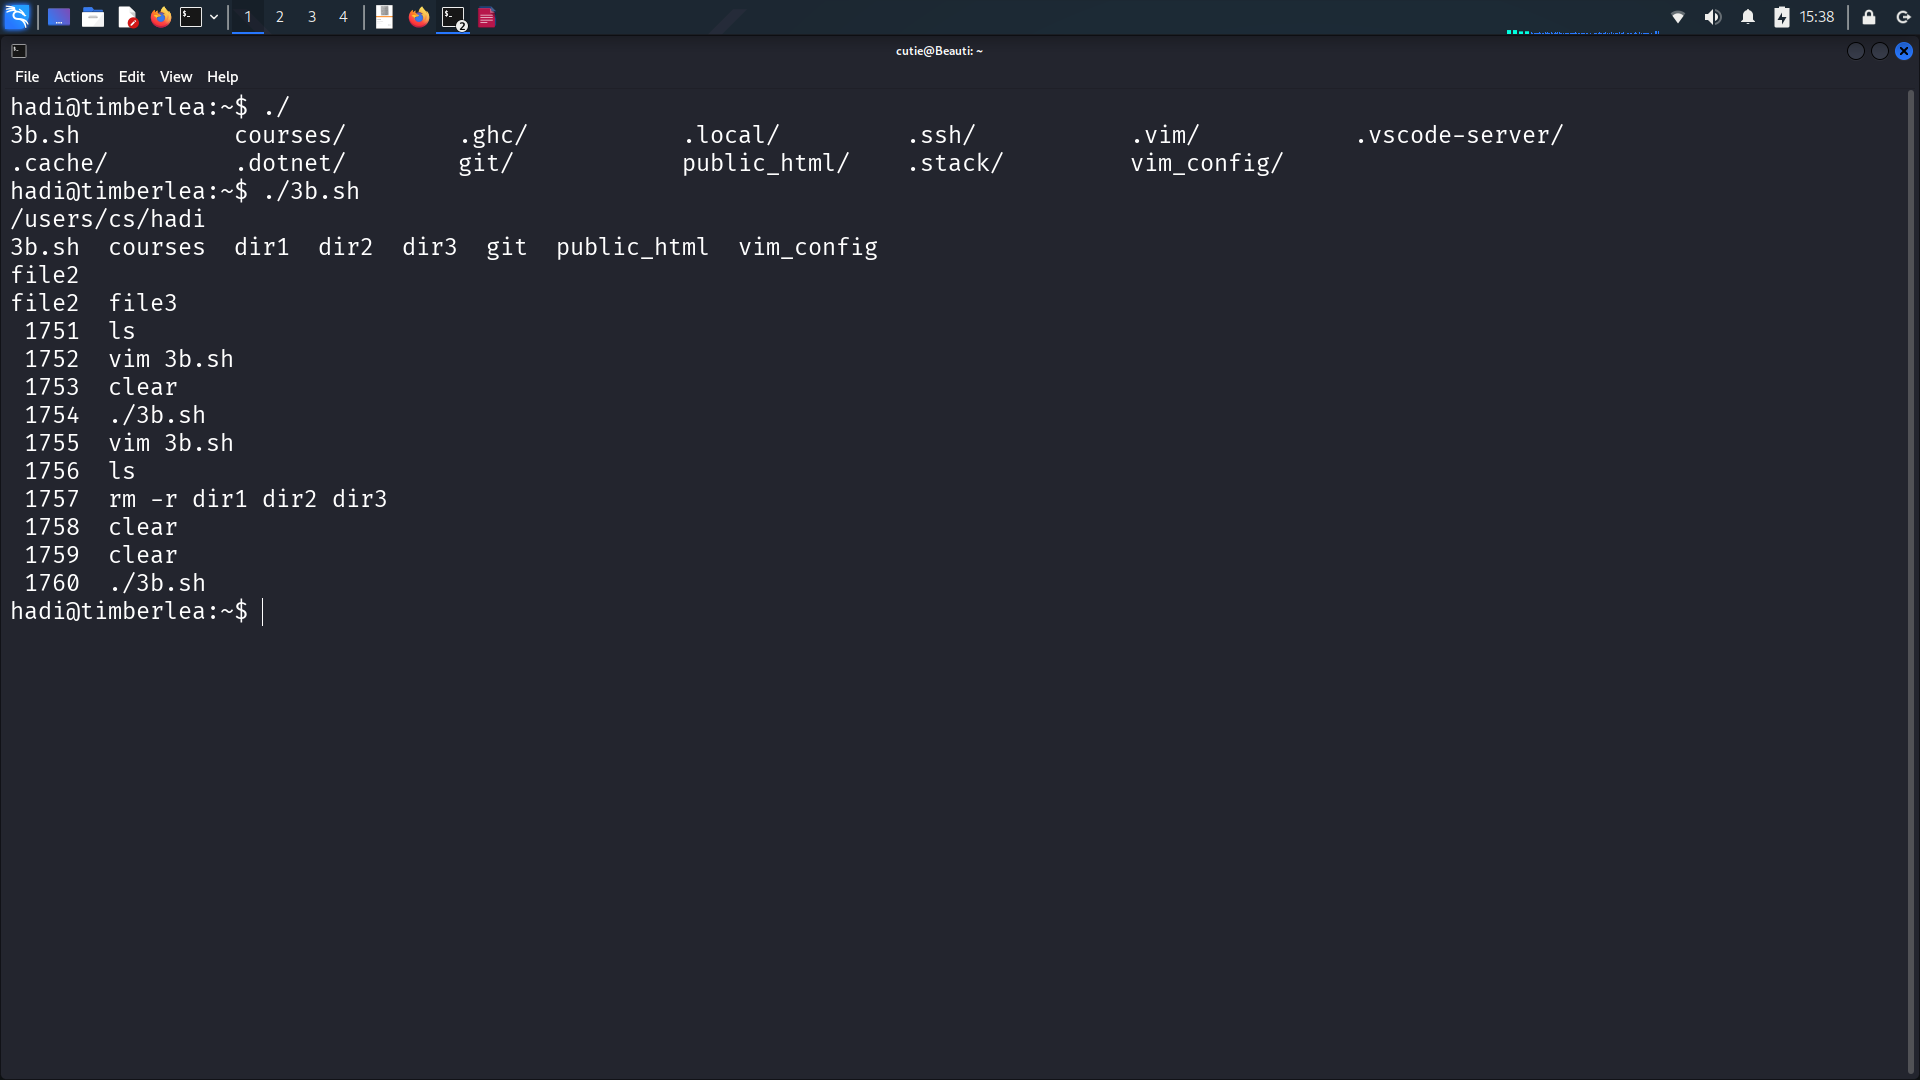
\includegraphics[width=400pt]{images/3b.png}
	\end{figure}

	\vspace{10pt}
	\textbf{Were the outputs different:}
	\par{
		No, the output was the same
	}

	\textbf{Why/why not to write a script:}
	
	\par{
		We want to write scripts for complex and repetitive tasks. So no, I probably would not
		write a script to run basic commands (such as ls, rm ...). Scripts are better
		suited for longer commands for example recompiling a C program with 
		external dependancies which would look something like:
		\begin{center}
			
		gcc -std=c18 (long list of .c) -I/(path to library)/include -o exec -(some more flags)
		\end{center}
		In this case you would write a Makefile (or a shell script)

	}
\end{document}
